\documentclass[11pt,a4paper]{article}

% ---- packages ----
\usepackage[utf8]{inputenc}
\usepackage[T1]{fontenc}
\usepackage{lmodern}
\usepackage{amsmath,amssymb,amsthm}
\usepackage{mathtools}
\usepackage{stmaryrd}
\usepackage{listings}
\usepackage{xcolor}
\usepackage{hyperref}
\usepackage{cleveref}
\usepackage{geometry}
\usepackage{booktabs}
\usepackage{enumitem}
\usepackage{tikz}
\usetikzlibrary{arrows.meta,positioning,shapes,calc,fit}
\usepackage{tikz-cd}
\usepackage{float}
\usepackage{caption}
\usepackage{subcaption}
\usepackage{fancyhdr}
\usepackage{natbib}
\usepackage{url}
\usepackage{microtype}
\usepackage{graphicx}

\geometry{margin=1in}

% ---- theorem environments ----
\newtheorem{theorem}{Theorem}[section]
\newtheorem{lemma}[theorem]{Lemma}
\newtheorem{proposition}[theorem]{Proposition}
\newtheorem{corollary}[theorem]{Corollary}
\newtheorem{definition}[theorem]{Definition}
\newtheorem{example}[theorem]{Example}
\newtheorem{remark}[theorem]{Remark}

% ---- listings configuration ----
\definecolor{japlkw}{RGB}{0,100,180}
\definecolor{japlstr}{RGB}{180,60,20}
\definecolor{japlcmt}{RGB}{100,130,100}
\definecolor{japltype}{RGB}{140,50,140}
\definecolor{codebg}{RGB}{248,248,248}

\lstdefinelanguage{japl}{
  keywords={fn,let,match,with,type,if,then,else,module,import,use,
            supervisor,strategy,child,test,assert,forall,
            receive,send,spawn,done,continue,fail,
            loop,while,do,where,opaque,signature,impl,trait,
            foreign,unsafe,own,ref,packed,deriving},
  keywordstyle=\color{japlkw}\bfseries,
  keywords=[2]{Int,Float,Bool,String,Bytes,Unit,Never,Option,Result,
               List,Map,Set,Pid,Reply,Process,Io,Net,State,Fail,Async,
               Pure,Ok,Err,Some,None,True,False,
               OneForOne,AllForOne,RestForOne,
               Permanent,Transient,Temporary,Normal},
  keywordstyle=[2]\color{japltype},
  sensitive=true,
  morecomment=[l]{--},
  morestring=[b]",
  commentstyle=\color{japlcmt}\itshape,
  stringstyle=\color{japlstr},
  basicstyle=\ttfamily\small,
  breaklines=true,
  showstringspaces=false,
  tabsize=2,
  backgroundcolor=\color{codebg},
  frame=single,
  framerule=0.4pt,
  rulecolor=\color{gray!40},
  xleftmargin=2em,
  framexleftmargin=1.5em,
  numbers=left,
  numberstyle=\tiny\color{gray},
  numbersep=8pt,
}

\lstdefinelanguage{erlang}{
  keywords={-module,-export,-behaviour,-callback,
            receive,after,end,case,of,when,fun,if,
            spawn,spawn_link,self,send,
            init,handle_call,handle_cast,handle_info,terminate},
  keywordstyle=\color{japlkw}\bfseries,
  sensitive=true,
  morecomment=[l]{\%},
  morestring=[b]",
  commentstyle=\color{japlcmt}\itshape,
  stringstyle=\color{japlstr},
  basicstyle=\ttfamily\small,
  breaklines=true,
  showstringspaces=false,
  tabsize=2,
  backgroundcolor=\color{codebg},
  frame=single,
  framerule=0.4pt,
  rulecolor=\color{gray!40},
  xleftmargin=2em,
  framexleftmargin=1.5em,
  numbers=left,
  numberstyle=\tiny\color{gray},
  numbersep=8pt,
}

\lstdefinelanguage{golang}{
  keywords={func,go,chan,select,case,default,make,range,
            for,if,else,return,var,type,struct,interface,
            defer,close,package,import},
  keywordstyle=\color{japlkw}\bfseries,
  sensitive=true,
  morecomment=[l]{//},
  morecomment=[s]{/*}{*/},
  morestring=[b]",
  morestring=[b]`,
  commentstyle=\color{japlcmt}\itshape,
  stringstyle=\color{japlstr},
  basicstyle=\ttfamily\small,
  breaklines=true,
  showstringspaces=false,
  tabsize=2,
  backgroundcolor=\color{codebg},
  frame=single,
  framerule=0.4pt,
  rulecolor=\color{gray!40},
  xleftmargin=2em,
  framexleftmargin=1.5em,
  numbers=left,
  numberstyle=\tiny\color{gray},
  numbersep=8pt,
}

\lstset{defaultdialect=[]{japl}}

% ---- process calculus macros ----
\newcommand{\piproc}{\pi}
\newcommand{\ppar}{\;\|\;}
\newcommand{\pzero}{\mathbf{0}}
\newcommand{\prepl}{!}
\newcommand{\pnew}[1]{(\nu\, #1)}
\newcommand{\psend}[2]{\overline{#1}\langle #2 \rangle}
\newcommand{\precv}[2]{#1(#2)}
\newcommand{\pchoice}{\oplus}
\newcommand{\pbranch}{\mathbin{\&}}
\newcommand{\pguard}[2]{#1 \triangleright #2}
\newcommand{\bisim}{\sim}
\newcommand{\wbisim}{\approx}
\newcommand{\Proc}{\mathsf{Proc}}
\newcommand{\Msg}{\mathsf{Msg}}
\newcommand{\Pid}{\mathsf{Pid}}
\newcommand{\Sup}{\mathsf{Sup}}
\newcommand{\Mailbox}{\mathsf{Mailbox}}
\newcommand{\spawn}{\mathsf{spawn}}
\newcommand{\sendf}{\mathsf{send}}
\newcommand{\recvf}{\mathsf{receive}}
\newcommand{\donef}{\mathsf{done}}
\newcommand{\failf}{\mathsf{fail}}
\newcommand{\Cat}[1]{\mathbf{#1}}
\newcommand{\Set}{\Cat{Set}}
\newcommand{\Hom}{\mathrm{Hom}}
\newcommand{\op}{\mathrm{op}}
\newcommand{\id}{\mathrm{id}}

% ---- title ----
\title{\textbf{Concurrency Is Process-Based, Not Shared-Memory-First:}\\[6pt]
\Large Typed Processes, Supervised Mailboxes, and Categorical\\
Semantics in the JAPL Programming Language}

\author{Matthew Long\\
The JAPL Research Collaboration\\
YonedaAI Research Collective\\
Chicago, IL\\
\texttt{matthew@yonedaai.com}}

\date{March 2026}

\begin{document}

\maketitle

% ================================================================
% ABSTRACT
% ================================================================
\begin{abstract}
Shared-memory concurrency---mediated by locks, atomics, and transactional memory---has dominated mainstream language design for decades, yet it remains a prolific source of data races, deadlocks, priority inversion, and heisenbugs that resist testing and formal verification alike. We present the concurrency model of JAPL, a strict, typed, effect-aware functional language that adopts process-based concurrency as its \emph{sole} primitive for managing concurrent state. Every concurrent entity in JAPL is a lightweight, heap-isolated process that communicates exclusively through statically typed mailboxes. Supervision trees---drawn from the Erlang/OTP tradition but extended with static typing, declarative backoff, and typed crash reasons---are built into the language and runtime, providing compositional fault tolerance. We develop a formal framework grounding JAPL's process model in the $\pi$-calculus with session types, give categorical semantics via presheaf categories over a time category, and prove key properties including typed message safety, deadlock freedom under supervision discipline, and progress guarantees for well-typed process networks. Empirical comparisons with Erlang/OTP, Go, Akka, and Pony demonstrate that JAPL's typed process model catches a significant class of concurrency errors at compile time while preserving the scalability and fault-tolerance characteristics that have made process-based systems the backbone of telecommunications and distributed infrastructure.
\end{abstract}

\vspace{1em}
\noindent\textbf{Keywords:} process-based concurrency, typed mailboxes, supervision trees, session types, actor model, $\pi$-calculus, effect systems, functional programming, fault tolerance

\newpage
\tableofcontents
\newpage

% ================================================================
% 1. INTRODUCTION
% ================================================================
\section{Introduction}\label{sec:intro}

The past two decades have witnessed an extraordinary expansion in concurrent and distributed computing. Multi-core processors are universal, cloud services routinely span thousands of nodes, and applications are expected to remain responsive under load while tolerating partial failures gracefully. Yet the dominant programming model for concurrency---shared mutable memory protected by locks---has failed to keep pace with these demands.

\subsection{The Shared-Memory Crisis}

Shared-memory concurrency is notoriously difficult to reason about. The fundamental problem is compositional: two correct, independently developed components, when composed in a shared-memory setting, may exhibit behaviors that neither component exhibits in isolation. This failure of compositionality manifests in several well-known pathologies:

\begin{description}[leftmargin=2em]
\item[Data races.] When two threads access the same memory location concurrently and at least one access is a write, the resulting behavior is undefined in languages like C and C++, and merely unpredictable in languages with a defined memory model like Java~\citep{manson2005java}. Data races are notoriously difficult to reproduce, diagnose, and test.

\item[Deadlocks.] Lock-based synchronization creates the possibility of circular wait conditions. The classic Coffman conditions~\citep{coffman1971system} are necessary and sufficient, but preventing them in practice requires either global lock ordering disciplines that do not compose, or detection mechanisms that add runtime overhead.

\item[Priority inversion.] When a low-priority thread holds a lock needed by a high-priority thread, the high-priority thread is effectively demoted. The Mars Pathfinder incident~\citep{reeves1997mars} demonstrated that this pathology can affect even carefully engineered real-time systems.

\item[Livelock and starvation.] Optimistic concurrency schemes based on compare-and-swap (CAS) operations can livelock under contention, and lock-free data structures, while avoiding deadlock, introduce their own complexity around memory reclamation (the ABA problem) and progress guarantees~\citep{michael2004hazard}.

\item[Memory model subtleties.] Modern hardware memory models are weak: processors reorder loads and stores, caches introduce visibility delays, and compilers perform optimizations that assume single-threaded execution. The resulting ``memory model'' specifications (e.g., the Java Memory Model~\citep{manson2005java}, the C++11 memory model~\citep{boehm2008foundations}) are themselves a source of bugs, as even experts routinely misunderstand the guarantees provided~\citep{sewell2010x86}.
\end{description}

\subsection{The Process Alternative}

An alternative tradition, originating in Hoare's Communicating Sequential Processes (CSP)~\citep{hoare1978communicating}, Milner's Calculus of Communicating Systems (CCS)~\citep{milner1980calculus} and $\pi$-calculus~\citep{milner1992calculus}, and Hewitt's Actor model~\citep{hewitt1973universal}, proposes a fundamentally different approach: concurrent entities do not share memory. Instead, they are isolated processes that communicate by passing messages. This model has been realized most successfully in Erlang/OTP~\citep{armstrong2003making}, which has powered telecommunications infrastructure with ``nine nines'' (99.9999999\%) availability for over three decades.

The process-based model eliminates data races \emph{by construction}: there is no shared mutable state to race on. Deadlocks are addressed not by prevention but by \emph{supervision}: if a process gets stuck or crashes, its supervisor detects the failure and takes corrective action (typically restarting the process with fresh state). This approach treats failures as normal, expected events rather than exceptional catastrophes---a philosophy that aligns with the reality of large-scale distributed systems.

\subsection{Contributions}

JAPL adopts process-based concurrency as its core model, but extends the Erlang tradition with insights from modern type theory:

\begin{enumerate}
\item \textbf{Typed mailboxes}: every process has a statically typed mailbox, preventing a large class of message-protocol errors at compile time (\Cref{sec:typed-mailboxes}).

\item \textbf{Typed supervision trees}: supervision strategies, restart policies, and crash reasons are integrated into the type system, enabling compositional reasoning about fault tolerance (\Cref{sec:supervision}).

\item \textbf{Effect-tracked concurrency}: the \texttt{Process} effect integrates with JAPL's effect system, making concurrency operations visible in function signatures and enabling safe composition with pure code (\Cref{sec:process-model}).

\item \textbf{Formal foundations}: we provide categorical semantics for JAPL's process model using presheaf categories over time, connect typed mailboxes to session types, and prove typed message safety and deadlock freedom (\Cref{sec:formal,sec:properties}).

\item \textbf{Implementation}: we describe a work-stealing scheduler, per-process heaps, and mailbox data structures that achieve Erlang-class scalability (millions of processes per node) with stronger static guarantees (\Cref{sec:implementation}).
\end{enumerate}

The remainder of this paper is organized as follows. \Cref{sec:background} surveys related work in concurrent language design and process calculi. \Cref{sec:formal} develops the formal framework. \Cref{sec:process-model} presents JAPL's process model in detail. \Cref{sec:typed-mailboxes} describes typed mailboxes. \Cref{sec:supervision} covers supervision trees. \Cref{sec:lifecycle} defines the process lifecycle. \Cref{sec:comparison} compares JAPL with existing approaches. \Cref{sec:implementation} discusses implementation. \Cref{sec:properties} proves formal properties. \Cref{sec:discussion} discusses limitations and future work. \Cref{sec:conclusion} concludes.


% ================================================================
% 2. BACKGROUND AND RELATED WORK
% ================================================================
\section{Background and Related Work}\label{sec:background}

\subsection{The Actor Model}

The Actor model, introduced by Hewitt, Bishop, and Steiger~\citep{hewitt1973universal} and formalized by Agha~\citep{agha1986actors}, posits that the fundamental unit of computation is the \emph{actor}: an entity that, in response to a message, can (1) send a finite number of messages to other actors, (2) create a finite number of new actors, and (3) designate the behavior to be used for the next message it receives. Actors encapsulate state and communicate exclusively through asynchronous message passing.

The Actor model provides a clean mathematical foundation for concurrency, but its original formulation leaves several practical questions open: how are actors supervised? How are message types enforced? How are actors distributed across nodes? JAPL's process model can be seen as a \emph{typed, supervised} refinement of the Actor model, informed by three decades of practical experience with Erlang/OTP.

\subsection{Communicating Sequential Processes}

Hoare's CSP~\citep{hoare1978communicating,roscoe1998theory} models concurrent systems as processes that communicate through \emph{synchronous} channels. Unlike the Actor model, CSP communication is rendezvous-based: both sender and receiver must be ready simultaneously. CSP's algebraic framework---with operators for sequential composition, parallel composition, choice, and hiding---enables powerful equational reasoning about concurrent systems.

CSP's synchronous semantics make it well-suited to modeling hardware and tightly-coupled concurrent systems, but less natural for distributed systems where asynchronous communication is the norm. Go's goroutines and channels~\citep{pike2012concurrency} are a practical realization of CSP ideas, though without the formal algebraic framework.

\subsection{The Pi-Calculus}

Milner's $\pi$-calculus~\citep{milner1992calculus,milner1999communicating} extends CCS~\citep{milner1980calculus} with \emph{name passing}: channel names themselves can be communicated, enabling the modeling of systems with dynamic communication topologies. The $\pi$-calculus has become the standard formal foundation for concurrent and mobile computation.

The key constructs of the $\pi$-calculus are:
\begin{align}
P, Q ::= \quad & \psend{x}{y}.P && \text{(output: send $y$ on channel $x$)} \notag \\
\mid \quad & \precv{x}{y}.P && \text{(input: receive $y$ on channel $x$)} \notag \\
\mid \quad & P \ppar Q && \text{(parallel composition)} \notag \\
\mid \quad & \pnew{x} P && \text{(restriction: create fresh channel $x$)} \notag \\
\mid \quad & \prepl P && \text{(replication)} \notag \\
\mid \quad & \pzero && \text{(inaction)} \notag
\end{align}

The $\pi$-calculus, equipped with typed channels~\citep{vasconcelos1998language}, provides the formal backbone for JAPL's typed mailbox system, as we develop in \Cref{sec:formal}.

\subsection{Erlang/OTP}

Erlang~\citep{armstrong2003making,armstrong2007programming} is the most successful realization of process-based concurrency in a general-purpose programming language. The BEAM virtual machine supports millions of lightweight processes per node, each with its own heap and mailbox. The OTP framework provides supervision trees, generic server behaviors, and a rich set of patterns for building fault-tolerant distributed systems.

Erlang's primary limitation, from the perspective of JAPL's design, is its dynamic type system. Messages are untyped: any term can be sent to any process, and protocol violations are detected only at runtime (if at all). This means that a large class of errors---sending the wrong message type to a process, forgetting to handle a message variant, protocol state machine violations---cannot be caught by the compiler. Dialyzer~\citep{lindahl2006practical} provides optional type annotations and success typing, but its analysis is necessarily conservative and cannot enforce the full range of protocol invariants that session types provide.

\subsection{Go: Goroutines and Channels}

Go~\citep{pike2012concurrency,donovan2015go} takes CSP-inspired channels as its concurrency primitive. Goroutines are lightweight threads multiplexed onto OS threads, and channels provide typed, synchronous (or buffered) communication. Go's concurrency model is syntactically lightweight and practically effective.

However, Go does not enforce process isolation: goroutines can (and routinely do) share memory. The \texttt{go vet} tool and the race detector~\citep{serebryany2012threadsanitizer} catch some data races dynamically, but Go does not prevent them statically. Go also lacks supervision: a panicking goroutine crashes the entire program unless manually recovered with \texttt{defer}/\texttt{recover}. There is no built-in mechanism for monitoring goroutine health or automatically restarting failed computations.

\subsection{Akka: Actors on the JVM}

Akka~\citep{lightbend2023akka} implements the Actor model on the JVM, providing location-transparent actors, supervision, and cluster sharding. Akka Typed~\citep{roestenburg2016akka} introduced typed actor references, partially addressing the message-typing problem. However, Akka operates within the JVM ecosystem, which means actors share a heap and can bypass the actor abstraction via shared mutable state. Supervision in Akka is a library concern rather than a language primitive, and the complexity of the JVM class hierarchy adds substantial cognitive overhead.

\subsection{Pony: Reference Capabilities}

Pony~\citep{clebsch2015deny} takes a novel approach to actor safety through \emph{reference capabilities}: a system of permissions (iso, val, ref, box, tag, trn) that statically guarantee data-race freedom. Pony actors communicate by passing messages, with the type system ensuring that mutable data is never aliased across actors. This is a powerful approach, but the cognitive burden of managing reference capabilities is significant, and the language has not achieved widespread adoption.

\subsection{Session Types}

Session types, introduced by Honda~\citep{honda1993types} and developed extensively by Honda, Vasconcelos, and Kubo~\citep{honda1998language}, Caires and Pfenning~\citep{caires2010session}, and Wadler~\citep{wadler2012propositions}, provide a type-theoretic framework for specifying and verifying communication protocols. A session type describes the sequence of messages exchanged between two parties, including message types, directions, branching, and recursion.

The Curry-Howard correspondence between linear logic and session types~\citep{caires2010session,wadler2012propositions} provides a deep theoretical foundation: propositions in linear logic correspond to session types, proofs correspond to processes, and cut elimination corresponds to communication. JAPL's typed mailboxes draw on this tradition, adapting multiparty session types~\citep{honda2008multiparty} to the supervision context.

\subsection{The E Language and Capability-Based Security}

The E programming language~\citep{miller2006robust} pioneered capability-based security in the context of distributed object computing. E's ``eventually'' references and promise pipelining influenced JAPL's approach to asynchronous communication, while its capability discipline informs JAPL's integration of process spawning with the capability type system.

\subsection{Gleam: Typed Erlang}

Gleam~\citep{gleam2023} compiles to Erlang bytecode and provides static typing for the BEAM ecosystem. Gleam's approach validates the thesis that adding types to Erlang-style concurrency is both possible and valuable, but Gleam inherits BEAM's runtime semantics wholesale rather than co-designing the type system and runtime as JAPL does.


% ================================================================
% 3. FORMAL FRAMEWORK
% ================================================================
\section{Formal Framework}\label{sec:formal}

We develop a formal framework for JAPL's process model that draws on three traditions: process algebra (providing operational semantics), type theory (providing static guarantees), and category theory (providing compositional semantics).

\subsection{Process Algebra Foundation}

We define a typed $\pi$-calculus variant, $\pi_{\text{JAPL}}$, that captures JAPL's process primitives.

\begin{definition}[Syntax of $\pi_{\text{JAPL}}$]\label{def:syntax}
The processes of $\pi_{\text{JAPL}}$ are defined by the grammar:
\begin{align}
P, Q ::= \quad & \spawn{x}{A}{P}{Q} && \text{spawn process $P$ at name $x$ with type $A$, continue as $Q$} \notag \\
\mid \quad & \sendf{x}{v}.P && \text{send value $v$ on channel $x$, continue as $P$} \notag \\
\mid \quad & \recvf{x}{y}.P && \text{receive value $y$ from mailbox of $x$, continue as $P$} \notag \\
\mid \quad & P \ppar Q && \text{parallel composition} \notag \\
\mid \quad & \pnew{x : A} P && \text{create fresh typed channel} \notag \\
\mid \quad & \donef && \text{successful termination} \notag \\
\mid \quad & \failf{r} && \text{failure with reason $r$} \notag \\
\mid \quad & \Sup{s}{\overline{P_i}} && \text{supervision with strategy $s$ over children $P_i$} \notag \\
\mid \quad & \mathsf{match}\; v\; \{\overline{p_i \Rightarrow P_i}\} && \text{pattern matching on received messages} \notag
\end{align}
\end{definition}

\begin{definition}[Message types]\label{def:msgtypes}
A message type $A$ in $\pi_{\text{JAPL}}$ is an algebraic data type:
\[
A ::= \sum_{i \in I} C_i(\overline{T_i})
\]
where each $C_i$ is a constructor and $\overline{T_i}$ is a sequence of payload types. The special type $\mathsf{Reply}[T]$ represents a one-shot reply channel carrying values of type $T$.
\end{definition}

\begin{definition}[Typing contexts]\label{def:typing}
A typing context $\Gamma$ maps channel names to message types:
\[
\Gamma ::= \emptyset \mid \Gamma, x : \Pid[A]
\]
where $\Pid[A]$ is the type of a process identifier whose mailbox accepts messages of type $A$.
\end{definition}

\subsection{Operational Semantics}

We give a labeled transition system (LTS) for $\pi_{\text{JAPL}}$.

\begin{definition}[Reduction rules]\label{def:reduction}
The reduction relation $\rightarrow$ is the smallest relation satisfying:

\begin{description}
\item[R-Comm:] Communication between a sender and a receiver:
\[
\sendf{x}{v}.P \ppar \recvf{x}{y}.Q \;\rightarrow\; P \ppar Q[v/y]
\]

\item[R-Spawn:] Process creation:
\[
\spawn{x}{A}{P}{Q} \;\rightarrow\; \pnew{x : \Pid[A]}(P \ppar Q)
\]

\item[R-Match:] Pattern matching on a received message $v = C_j(\overline{w})$:
\[
\mathsf{match}\; C_j(\overline{w})\; \{\overline{C_i(\overline{y_i}) \Rightarrow P_i}\} \;\rightarrow\; P_j[\overline{w}/\overline{y_j}]
\]

\item[R-Fail:] Failure propagation under supervision:
\[
\Sup{s}{P_1 \ppar \cdots \ppar \failf{r} \ppar \cdots \ppar P_n} \;\rightarrow\; \mathsf{restart}(s, r, \overline{P_i})
\]
where $\mathsf{restart}$ applies the supervision strategy $s$.

\item[R-Par:] Structural rule for parallel composition:
\[
\frac{P \rightarrow P'}{P \ppar Q \rightarrow P' \ppar Q}
\]

\item[R-New:] Structural rule for restriction:
\[
\frac{P \rightarrow P'}{\pnew{x:A} P \rightarrow \pnew{x:A} P'}
\]
\end{description}
\end{definition}

\subsection{Type System}

\begin{definition}[Typing judgment]\label{def:typejudge}
The typing judgment $\Gamma \vdash P$ asserts that process $P$ is well-typed under context $\Gamma$. The key rules are:

\begin{description}
\item[T-Send:]
\[
\frac{\Gamma \vdash x : \Pid[A] \quad \Gamma \vdash v : A \quad \Gamma \vdash P}{\Gamma \vdash \sendf{x}{v}.P}
\]

\item[T-Recv:]
\[
\frac{\Gamma, y : A \vdash P \quad \Gamma \vdash \mathsf{self} : \Pid[A]}{\Gamma \vdash \recvf{\mathsf{self}}{y}.P}
\]

\item[T-Spawn:]
\[
\frac{\Gamma, x : \Pid[A] \vdash P : \mathsf{Process}[A] \quad \Gamma, x : \Pid[A] \vdash Q}{\Gamma \vdash \spawn{x}{A}{P}{Q}}
\]

\item[T-Sup:]
\[
\frac{s : \mathsf{Strategy} \quad \forall i.\; \Gamma \vdash P_i}{\Gamma \vdash \Sup{s}{\overline{P_i}}}
\]
\end{description}
\end{definition}

\subsection{Categorical Semantics}

We provide denotational semantics for $\pi_{\text{JAPL}}$ using category theory, following the tradition of presheaf models for concurrency~\citep{joyal1996bisimulation,cattani1997presheaf}.

\begin{definition}[Time category]\label{def:timecat}
Let $\Cat{T}$ be the category whose objects are natural numbers (representing discrete time steps) and whose morphisms $m \leq n$ are the unique arrows witnessing $m \leq n$ in the natural order. This is the poset $(\mathbb{N}, \leq)$ viewed as a category.
\end{definition}

\begin{definition}[Process presheaf]\label{def:procpresheaf}
A \emph{process presheaf} is a functor $F : \Cat{T}^{\op} \to \Set$. For each time $t$, $F(t)$ is the set of possible states of the process at time $t$. For each $m \leq n$, the restriction map $F(m \leq n) : F(n) \to F(m)$ captures the idea that the state at time $n$ determines (by restriction) information about the state at time $m$.
\end{definition}

The following diagram illustrates how an internal $\tau$-reduction (a silent step that does not involve external communication) maps into the presheaf structure. A process in state $\sigma \in F(t)$ that performs a $\tau$-reduction transitions to state $\sigma' \in F(t+1)$, while the restriction map recovers the earlier state:

\begin{figure}[H]
\centering
\begin{tikzcd}[column sep=3.5cm, row sep=2cm]
F(t) \ar[d, "\text{restriction}"', "F(t \leq t{+}1)"{swap}] & \sigma \in F(t) \ar[d, mapsto] \ar[r, "\tau\text{-reduction}"] & \sigma' \in F(t{+}1) \ar[dl, dashed, "F(t \leq t{+}1)"{description}] \\
F(t) & \sigma &
\end{tikzcd}
\caption{$\tau$-reduction in the presheaf model. A silent transition advances the process from time $t$ to $t+1$. The restriction map $F(t \leq t{+}1)$ projects back, ensuring that the presheaf coherence condition $F(s \leq t) \circ F(t \leq u) = F(s \leq u)$ is maintained across all internal reductions.}
\label{fig:tau-presheaf}
\end{figure}

\begin{definition}[Typed process category]\label{def:typedproccat}
The category $\Cat{TProc}$ has:
\begin{itemize}
\item \textbf{Objects:} Pairs $(P, A)$ where $P$ is a process presheaf and $A$ is a message type.
\item \textbf{Morphisms:} $(P, A) \to (Q, B)$ are natural transformations $\alpha : P \Rightarrow Q$ together with a message translation function $f : A \to B$ such that the following diagram commutes for all times $t$:
\[
\begin{tikzcd}
P(t) \times A \ar[r, "\alpha_t \times f"] \ar[d, "\mathsf{recv}_P"] & Q(t) \times B \ar[d, "\mathsf{recv}_Q"] \\
P(t+1) \ar[r, "\alpha_{t+1}"] & Q(t+1)
\end{tikzcd}
\]
where $\mathsf{recv}$ denotes the message reception transition.
\end{itemize}
\end{definition}

\begin{proposition}[Yoneda embedding]\label{prop:yoneda}
The Yoneda embedding $\Cat{T} \hookrightarrow [\Cat{T}^{\op}, \Set]$ maps each time point $t$ to the representable presheaf $\Hom_{\Cat{T}}(-, t)$. A process $P$ at time $t$ is characterized by the natural transformations $\Hom_{\Cat{T}}(-, t) \Rightarrow P$, which by the Yoneda lemma are in bijection with elements of $P(t)$---i.e., the states of the process at time $t$.
\end{proposition}

\begin{definition}[Communication as profunctor]\label{def:profunctor}
A \emph{communication channel} between process categories $\Cat{C}$ and $\Cat{D}$ is a profunctor $H : \Cat{C}^{\op} \times \Cat{D} \to \Set$. For processes $c \in \Cat{C}$ and $d \in \Cat{D}$, the set $H(c, d)$ represents the possible messages that can flow from $c$ to $d$. Typed mailboxes correspond to profunctors $H$ that factor through the message type:
\[
H(c, d) = \Hom_A(\mathsf{out}(c), \mathsf{in}(d))
\]
where $\mathsf{out}(c)$ and $\mathsf{in}(d)$ are the output and input types of $c$ and $d$ respectively, and $\Hom_A$ is the hom-set in the category of message types.
\end{definition}

\subsubsection{Connecting Categorical and Operational Semantics}

The categorical semantics developed above relate to the $\pi_{\text{JAPL}}$ operational semantics (\Cref{def:reduction}) through a denotational--operational bridge. Every well-typed $\pi_{\text{JAPL}}$ process $P$ with mailbox type $A$ induces a process presheaf $\llbracket P \rrbracket \in \Cat{TProc}$, where $\llbracket P \rrbracket(t)$ is the set of reachable states of $P$ after exactly $t$ reduction steps. The restriction maps $\llbracket P \rrbracket(m \leq n) : \llbracket P \rrbracket(n) \to \llbracket P \rrbracket(m)$ are well-defined because every state reachable in $n$ steps determines (by truncating the reduction trace) the state at step $m$. \emph{Soundness} asserts that if two processes are identified in the categorical model---i.e., their presheaves are naturally isomorphic in $\Cat{TProc}$---then they are typed-bisimilar in the operational semantics: $\llbracket P \rrbracket \cong \llbracket Q \rrbracket$ implies $(P,A) \bisim (Q,A)$. This follows because a natural isomorphism between presheaves preserves the $\mathsf{recv}$ transition structure at every time step, which is exactly the transfer property required by typed bisimulation (\Cref{def:bisim}). \emph{Completeness} (the converse) holds for finite-state processes: if $(P,A) \bisim (Q,A)$, the bisimulation relation itself provides the components of a natural isomorphism $\llbracket P \rrbracket \cong \llbracket Q \rrbracket$. For infinite-state processes, completeness requires passing to the coalgebraic completion of $\Cat{TProc}$, which we leave to future work. Together, these results ensure that reasoning in the categorical model faithfully reflects the operational behavior of $\pi_{\text{JAPL}}$ programs.

\subsection{Bisimulation}

\begin{definition}[Typed bisimulation]\label{def:bisim}
A \emph{typed bisimulation} is a relation $\mathcal{R}$ on typed processes such that if $(P, A) \mathcal{R} (Q, A)$ (note: same message type), then:
\begin{enumerate}
\item If $P \xrightarrow{\tau} P'$, then there exists $Q'$ such that $Q \xrightarrow{\tau} Q'$ and $(P', A) \mathcal{R} (Q', A)$.
\item If $P \xrightarrow{\recvf{}{v}} P'$ where $v : A$, then there exists $Q'$ such that $Q \xrightarrow{\recvf{}{v}} Q'$ and $(P', A) \mathcal{R} (Q', A)$.
\item Symmetrically for $Q$.
\end{enumerate}
Two typed processes are \emph{bisimilar}, written $(P, A) \bisim (Q, A)$, if there exists a typed bisimulation relating them.
\end{definition}

\begin{theorem}[Congruence]\label{thm:congruence}
Typed bisimilarity is a congruence with respect to all $\pi_{\text{JAPL}}$ constructors: parallel composition, restriction, supervision, and spawning.
\end{theorem}

\begin{proof}[Proof sketch]
The proof proceeds by showing that for each constructor $\mathcal{C}$, if $(P, A) \bisim (Q, A)$ then $(\mathcal{C}[P], A') \bisim (\mathcal{C}[Q], A')$ for the appropriate type $A'$. The key insight is that typed bisimulation respects message types: substituting bisimilar processes in any context preserves the ability to send and receive the same typed messages. The supervision case requires showing that if $P \bisim Q$ and both crash with the same typed reason, then their restarts (under any strategy) are also bisimilar.
\end{proof}


% ================================================================
% 4. JAPL'S PROCESS MODEL
% ================================================================
\section{JAPL's Process Model}\label{sec:process-model}

JAPL's concurrency model is built on a single primitive: the \emph{process}. A process is a lightweight, isolated unit of concurrent execution with the following properties:

\begin{enumerate}
\item \textbf{Isolated state:} Each process has its own heap. There is no shared mutable memory between processes. Pure immutable values may be shared (they are safe to share because they cannot change), but mutable resources are owned by exactly one process at a time.

\item \textbf{Typed mailbox:} Each process has a single mailbox that accepts messages of a statically known type. The type system prevents sending a message of the wrong type.

\item \textbf{Supervision relationship:} Every process (except the root) has a supervisor. If a process crashes, its supervisor is notified and takes corrective action according to a declared strategy.

\item \textbf{Location transparency:} Process identifiers ($\Pid[A]$) are location-transparent. A PID may refer to a process on the local node or a remote node; the runtime handles serialization, routing, and network transport.

\item \textbf{Effect tracking:} Process operations (spawn, send, receive) are tracked by the effect system. A function that performs process operations must declare the $\mathsf{Process}[A]$ effect in its signature.
\end{enumerate}

\subsection{Process Isolation}

The cornerstone of JAPL's concurrency safety is process isolation. Unlike Go (where goroutines share memory), Java (where threads share the heap), or even Akka (where JVM actors can access shared objects), JAPL enforces isolation through a combination of language semantics and runtime architecture:

\begin{lstlisting}[language=japl,caption={Process isolation: no shared mutable state}]
-- Each process has its own state, managed via recursion
fn worker(state: WorkerState) -> Never with Process[WorkerMsg] =
  match Process.receive() with
  | DoWork(task, reply) ->
      -- state is local to this process; no other process can access it
      let result = execute_task(state, task)
      let new_state = update_state(state, task, result)
      Reply.send(reply, result)
      worker(new_state)  -- tail-recursive loop with new state
  | Shutdown ->
      cleanup(state)
      Process.exit(Normal)
\end{lstlisting}

The key mechanisms ensuring isolation are:

\begin{description}
\item[Immutable sharing.] Pure values (algebraic data types, records, strings, lists) are immutable and can be shared across process boundaries without copying or synchronization. Since they cannot change, concurrent access is inherently safe.

\item[Ownership transfer.] Mutable resources (file handles, buffers, network sockets) are governed by JAPL's ownership type system. A resource has exactly one owner. To pass a mutable resource to another process, ownership must be explicitly transferred, at which point the sending process can no longer access it:
\begin{lstlisting}[language=japl,caption={Ownership transfer between processes}]
fn send_to_worker(buf: own Buffer, pid: Pid[WorkerMsg]) -> Unit =
  Process.send(pid, ProcessBuffer(buf))
  -- buf is moved; using it here is a compile error
\end{lstlisting}

\item[Per-process heaps.] The runtime allocates a separate heap for each process. Garbage collection of one process's heap does not pause other processes. When a process terminates, its entire heap is reclaimed instantly.
\end{description}

\subsection{The Process Effect}

Concurrency in JAPL is not ambient: it is tracked by the effect system. Any function that spawns processes, sends messages, or receives messages must declare the $\mathsf{Process}[A]$ effect:

\begin{lstlisting}[language=japl,caption={The Process effect in function signatures}]
-- Pure function: no concurrency
fn calculate_price(item: Item, qty: Int) -> Money =
  Money.multiply(item.price, qty)

-- Process function: concurrency is declared
fn order_processor(state: State) -> Never with Process[OrderMsg] =
  match Process.receive() with
  | NewOrder(order) ->
      let priced = List.map(order.items, fn item ->
        { item | total = calculate_price(item, item.qty) }
      )
      order_processor({ state | pending = priced })
\end{lstlisting}

This has several benefits:
\begin{itemize}
\item Pure functions are guaranteed to be free of concurrency effects. They can be tested, reasoned about, and composed without concern for race conditions.
\item The effect system ensures that process operations cannot ``leak'' into pure code.
\item Effect polymorphism allows writing generic code that works in both pure and concurrent contexts.
\end{itemize}

\subsection{Message Passing Semantics}

JAPL's message passing is \emph{asynchronous} and \emph{reliable} for local processes:

\begin{description}
\item[Asynchronous send.] $\mathsf{Process.send}(pid, msg)$ enqueues $msg$ in the target process's mailbox and returns immediately. It never blocks the sender.

\item[Blocking receive.] $\mathsf{Process.receive}()$ blocks the calling process until a message is available in its mailbox. A timeout variant, $\mathsf{Process.receive\_with\_timeout}(ms)$, returns $\mathsf{Err}(\mathsf{Timeout})$ if no message arrives within the specified duration.

\item[Selective receive.] $\mathsf{Process.receive\_matching}(predicate)$ receives the first message in the mailbox that satisfies the predicate, leaving non-matching messages in the queue. This is essential for implementing protocols where messages may arrive out of order.

\item[Ordering guarantee.] Messages from a single sender to a single receiver are delivered in the order they were sent. No ordering is guaranteed between messages from different senders.
\end{description}

\begin{lstlisting}[language=japl,caption={Message passing primitives}]
type Msg =
  | StartJob(JobId)
  | CancelJob(JobId)
  | JobFinished(JobId, Output)
  | JobFailed(JobId, Reason)

fn worker_loop(state: WorkerState) -> Process<Unit> {
  receive {
    StartJob(id) =>
      worker_loop(begin_job(state, id))
    CancelJob(id) =>
      worker_loop(cancel_job(state, id))
    Shutdown =>
      done()
  }
}
\end{lstlisting}


% ================================================================
% 5. TYPED MAILBOXES
% ================================================================
\section{Typed Mailboxes}\label{sec:typed-mailboxes}

\subsection{Motivation}

In Erlang, any term can be sent to any process. The burden of message discrimination falls entirely on the receiving process, which must pattern-match on incoming messages and (hopefully) handle all possible cases. This design has served Erlang well for dynamically-typed, hot-code-reloading scenarios, but it has significant drawbacks:

\begin{enumerate}
\item \textbf{Protocol violations are silent.} Sending a message of the wrong type to a process does not cause an immediate error. The message sits in the mailbox, potentially forever (if no clause matches it), causing a slow memory leak and eventual process crash.

\item \textbf{Refactoring is dangerous.} Adding or removing a variant from a message type requires updating all senders---but the compiler provides no guidance on which senders to update.

\item \textbf{Documentation is informal.} The expected message protocol of a process is documented in comments or convention, not in the type system.
\end{enumerate}

\subsection{JAPL's Approach}

In JAPL, every process has a mailbox typed by an algebraic data type. The type of a process identifier, $\Pid[A]$, encodes the type of messages the process accepts:

\begin{lstlisting}[language=japl,caption={Typed mailbox definition and use}]
type LoggerMsg =
  | Log(Level, String)
  | Flush(Reply[Unit])
  | SetLevel(Level)

-- This process can ONLY receive LoggerMsg values
fn logger(config: LogConfig) -> Never with Process[LoggerMsg] =
  match Process.receive() with
  | Log(level, msg) ->
      if level >= config.min_level then
        write_log(config.output, level, msg)
      logger(config)
  | Flush(reply) ->
      flush_output(config.output)
      Reply.send(reply, ())
      logger(config)
  | SetLevel(level) ->
      logger({ config | min_level = level })

-- Spawning returns a typed PID
let pid: Pid[LoggerMsg] = Process.spawn(fn -> logger(default_config))

-- Type-safe sending: only LoggerMsg values are accepted
Process.send(pid, Log(Info, "server started"))
Process.send(pid, SetLevel(Debug))

-- Type error: wrong message type
-- Process.send(pid, "hello")     -- COMPILE ERROR
-- Process.send(pid, Increment)   -- COMPILE ERROR
\end{lstlisting}

\subsection{Contrast with Erlang}

Consider the equivalent Erlang code:

\begin{lstlisting}[language=erlang,caption={Erlang: untyped messages}]
logger(Config) ->
  receive
    {log, Level, Msg} ->
      case Level >= maps:get(min_level, Config) of
        true -> write_log(maps:get(output, Config), Level, Msg);
        false -> ok
      end,
      logger(Config);
    {flush, From} ->
      flush_output(maps:get(output, Config)),
      From ! ok,
      logger(Config);
    {set_level, Level} ->
      logger(Config#{min_level => Level})
    %% What happens if someone sends an unexpected message?
    %% It sits in the mailbox forever, leaking memory.
  end.
\end{lstlisting}

In Erlang, there is no compile-time check that senders use the correct tuple structure. A misspelling (\texttt{\{logmsg, info, "text"\}} instead of \texttt{\{log, info, "text"\}}) creates a silent failure.

\subsection{Reply Channels and Request-Response}

A common pattern in concurrent systems is request-response: a client sends a request and expects a reply. JAPL supports this through the $\mathsf{Reply}[T]$ type, which is a one-shot, typed reply channel:

\begin{lstlisting}[language=japl,caption={Request-response with typed reply channels}]
type CacheMsg =
  | Get(Key, Reply[Option[Value]])
  | Put(Key, Value)
  | Invalidate(Key)
  | Stats(Reply[CacheStats])

fn cache_server(store: Map[Key, Value]) -> Never with Process[CacheMsg] =
  match Process.receive() with
  | Get(key, reply) ->
      Reply.send(reply, Map.lookup(store, key))
      cache_server(store)
  | Put(key, value) ->
      cache_server(Map.insert(store, key, value))
  | Invalidate(key) ->
      cache_server(Map.delete(store, key))
  | Stats(reply) ->
      Reply.send(reply, compute_stats(store))
      cache_server(store)

-- Client-side: type-safe request-response
fn lookup_cached(pid: Pid[CacheMsg], key: Key) -> Option[Value] with Process =
  let reply = Reply.new()
  Process.send(pid, Get(key, reply))
  Reply.await(reply)  -- blocks until reply arrives; typed as Option[Value]
\end{lstlisting}

The $\mathsf{Reply}[T]$ type is \emph{affine} in implementation: it may be used \emph{at most once}, with a complementary liveness check that ensures it is used \emph{at least once} on every reachable code path. Together, these two checks enforce exactly-once semantics. JAPL does not require a full substructural type system; instead, $\mathsf{Reply}[T]$ values are tracked by a lightweight affine usage analysis integrated into the type checker. Each $\mathsf{Reply}[T]$ binding is marked as ``unconsumed'' at creation and ``consumed'' after a call to $\mathsf{Reply.send}$. A second use after consumption, or a path where the binding is never consumed, triggers a compile-time error. The following example illustrates the compile-time rejection of double use:

\begin{lstlisting}[language=japl,caption={Compile error: Reply used twice}]
fn bad_handler(state: State) -> Never with Process[CacheMsg] =
  match Process.receive() with
  | Get(key, reply) ->
      Reply.send(reply, Map.lookup(state.store, key))
      -- COMPILE ERROR: linear value 'reply' used after consumption
      Reply.send(reply, None)
      bad_handler(state)
\end{lstlisting}

Similarly, forgetting to reply in a branch is rejected:

\begin{lstlisting}[language=japl,caption={Compile error: Reply not consumed on all paths}]
fn forgetful_handler(state: State) -> Never with Process[CacheMsg] =
  match Process.receive() with
  | Get(key, reply) ->
      if Map.contains(state.store, key) then
        Reply.send(reply, Map.lookup(state.store, key))
        -- 'reply' consumed here
      else
        ()  -- COMPILE ERROR: linear value 'reply' not consumed on this path
      forgetful_handler(state)
\end{lstlisting}

This approach prevents a common class of bugs in actor systems---unanswered requests and duplicate replies---without imposing the full cognitive overhead of a substructural type system on all values.

\subsection{Session Types for Complex Protocols}

For protocols more complex than single request-response, JAPL supports session types~\citep{honda1993types} that describe multi-step communication sequences:

\begin{lstlisting}[language=japl,caption={Session-typed protocol}]
type AuthProtocol =
  session {
    client -> server: Credentials
    server -> client: AuthResult
    if authenticated:
      client -> server: Request
      server -> client: Response
    else:
      end
  }

-- The compiler verifies that both sides follow the protocol
fn auth_client(server: Pid[AuthProtocol.Server]) -> Result[Response, AuthError]
    with Process =
  let session = Session.connect(server)
  Session.send(session, my_credentials)
  match Session.receive(session) with
  | Authenticated(token) ->
      Session.send(session, my_request)
      let response = Session.receive(session)
      Ok(response)
  | Rejected(reason) ->
      Err(AuthFailed(reason))
\end{lstlisting}

Session types provide compile-time guarantees that:
\begin{itemize}
\item Messages are sent and received in the correct order.
\item Both parties agree on the types of messages at each step.
\item All protocol branches are handled.
\item Sessions are completed (no dangling sessions).
\end{itemize}

\subsection{Formal Typing of Mailboxes}

\begin{definition}[Mailbox typing rule]\label{def:mailbox-typing}
A process $P$ with mailbox type $A$ is well-typed, written $\Gamma \vdash_A P$, if:
\begin{enumerate}
\item Every $\recvf{\mathsf{self}}{y}.Q$ in $P$ binds $y$ at type $A$.
\item Every pattern match on a received message $y$ is exhaustive over the constructors of $A$.
\item Every $\sendf{x}{v}.Q$ where $\Gamma(x) = \Pid[B]$ has $v : B$.
\end{enumerate}
\end{definition}

\begin{theorem}[Typed message safety]\label{thm:msg-safety}
If $\Gamma \vdash P$ in $\pi_{\text{JAPL}}$, then during any execution of $P$, every message received by a process with mailbox type $A$ has type $A$.
\end{theorem}

\begin{proof}
By induction on the typing derivation and case analysis on the reduction rules. The key cases are:

\textbf{Case R-Comm:} The communication rule $\sendf{x}{v}.P \ppar \recvf{x}{y}.Q \rightarrow P \ppar Q[v/y]$ requires, by T-Send, that $v : A$ where $\Gamma(x) = \Pid[A]$, and by T-Recv, that $y$ is bound at type $A$. Therefore $Q[v/y]$ is well-typed.

\textbf{Case R-Spawn:} The spawn rule creates a new channel $x : \Pid[A]$. By T-Spawn, the spawned process has effect $\mathsf{Process}[A]$, so it receives messages of type $A$. The continuation can only send type-$A$ messages to $x$.

\textbf{Case R-Par:} By induction hypothesis on each component.

\textbf{Case R-New:} By induction hypothesis under the extended context.

The supervision case (R-Fail) preserves typing because the restart creates a fresh instance of the same process with the same type.
\end{proof}


% ================================================================
% 6. SUPERVISION TREES
% ================================================================
\section{Supervision Trees}\label{sec:supervision}

\subsection{Philosophy: Let It Crash}

Erlang's ``let it crash'' philosophy~\citep{armstrong2003making} is one of the most important insights in the history of concurrent programming. The idea is simple but profound: instead of trying to anticipate and handle every possible failure within a process, allow the process to crash and delegate recovery to a supervisor. This approach has several advantages:

\begin{enumerate}
\item \textbf{Simplicity.} Process code handles the ``happy path.'' It does not need defensive error handling for every possible corruption of state, hardware failure, or unexpected condition.

\item \textbf{Clean state.} Restarting a process gives it fresh, known-good state. This eliminates the problem of processes continuing with corrupted state after a partial failure.

\item \textbf{Isolation of failure.} A crash in one process does not corrupt the state of other processes. Supervision boundaries are fault boundaries.

\item \textbf{Compositionality.} Supervision trees compose: a supervisor can itself be supervised, creating hierarchical fault domains.
\end{enumerate}

JAPL adopts this philosophy and extends it with static typing.

\subsection{Supervision Strategies}

JAPL provides three supervision strategies, matching Erlang/OTP:

\begin{description}
\item[\texttt{OneForOne}:] When a child process crashes, only that child is restarted. Other children are unaffected. This is appropriate when children are independent.

\item[\texttt{AllForOne}:] When any child crashes, all children are terminated and restarted. This is appropriate when children have complex interdependencies and their collective state must be consistent.

\item[\texttt{RestForOne}:] When a child crashes, that child and all children started \emph{after} it are terminated and restarted. This is appropriate when children have a sequential dependency: later children depend on earlier ones.
\end{description}

\begin{lstlisting}[language=japl,caption={Supervisor declaration with typed crash reasons}]
supervisor ApiSystem {
  strategy: OneForOne
  child http_server()
  child metrics_reporter()
  child cache_manager()
}

-- Expanded form with full child specifications
fn start_app() -> Pid[SupervisorMsg] with Process =
  Supervisor.start(
    strategy = OneForOne,
    max_restarts = 5,
    max_seconds = 60,
    children = [
      { id = "db_pool"
      , start = fn -> DbPool.start(config.database)
      , restart = Permanent
      , shutdown = Timeout(5000)
      },
      { id = "http_server"
      , start = fn -> HttpServer.start(config.http)
      , restart = Permanent
      , shutdown = Timeout(10000)
      },
      { id = "background_jobs"
      , start = fn -> JobRunner.start(config.jobs)
      , restart = Transient
      , shutdown = Timeout(30000)
      },
    ]
  )
\end{lstlisting}

\subsection{Restart Policies}

Each child process has a restart policy:

\begin{description}
\item[\texttt{Permanent}:] Always restarted when it terminates, regardless of reason. Used for long-running services.
\item[\texttt{Transient}:] Restarted only if it terminates abnormally (crashes). Normal termination is not restarted. Used for tasks that may complete.
\item[\texttt{Temporary}:] Never restarted. Used for one-shot tasks.
\end{description}

\subsection{Restart Intensity and Backoff}

To prevent restart storms (where a persistently failing process is restarted in a tight loop, consuming resources), supervisors enforce a \emph{restart intensity}: a maximum number of restarts within a time window. If the intensity is exceeded, the supervisor itself crashes, propagating the failure up the supervision tree.

\begin{lstlisting}[language=japl,caption={Declarative backoff for restart intensity}]
supervisor DatabaseCluster {
  strategy: OneForOne
  max_restarts: 5
  max_seconds: 60
  backoff: Exponential { base_ms = 100, max_ms = 30000, jitter = True }

  child db_connection("primary", config.primary_url)
  child db_connection("replica-1", config.replica1_url)
  child db_connection("replica-2", config.replica2_url)
}
\end{lstlisting}

The \texttt{backoff} specification is a JAPL extension to the OTP model. Rather than immediately restarting a failed child, the supervisor waits for an exponentially increasing duration, with optional jitter to prevent thundering-herd effects. This is particularly valuable for processes that connect to external resources (databases, APIs), where immediate restart after a connection failure is unlikely to succeed.

\subsection{Typed Crash Reasons}

In Erlang, crash reasons are arbitrary terms. In JAPL, crash reasons are typed, enabling compile-time reasoning about failure modes:

\begin{lstlisting}[language=japl,caption={Typed crash reasons}]
type DbCrashReason =
  | ConnectionLost(String)
  | QueryTimeout(Duration)
  | ProtocolError(Bytes)
  | AuthenticationFailed

type HttpCrashReason =
  | BindFailed(Port)
  | TlsError(TlsErrorKind)
  | AcceptError(IoError)

-- Supervisor can pattern-match on typed crash reasons
fn on_child_crash(child_id: String, reason: CrashReason) -> SupervisorAction =
  match reason with
  | DbCrashReason(ConnectionLost(_)) ->
      Restart(Backoff(Exponential { base_ms = 500 }))
  | DbCrashReason(AuthenticationFailed) ->
      -- Don't restart; auth won't fix itself
      Escalate
  | HttpCrashReason(BindFailed(port)) ->
      Log.error("Port " ++ show(port) ++ " unavailable")
      Escalate
  | _ ->
      RestartImmediately
\end{lstlisting}

\subsection{Supervision Tree Visualization}

The supervision tree structure for a typical JAPL application is illustrated in \Cref{fig:suptree}.

\begin{figure}[H]
\centering
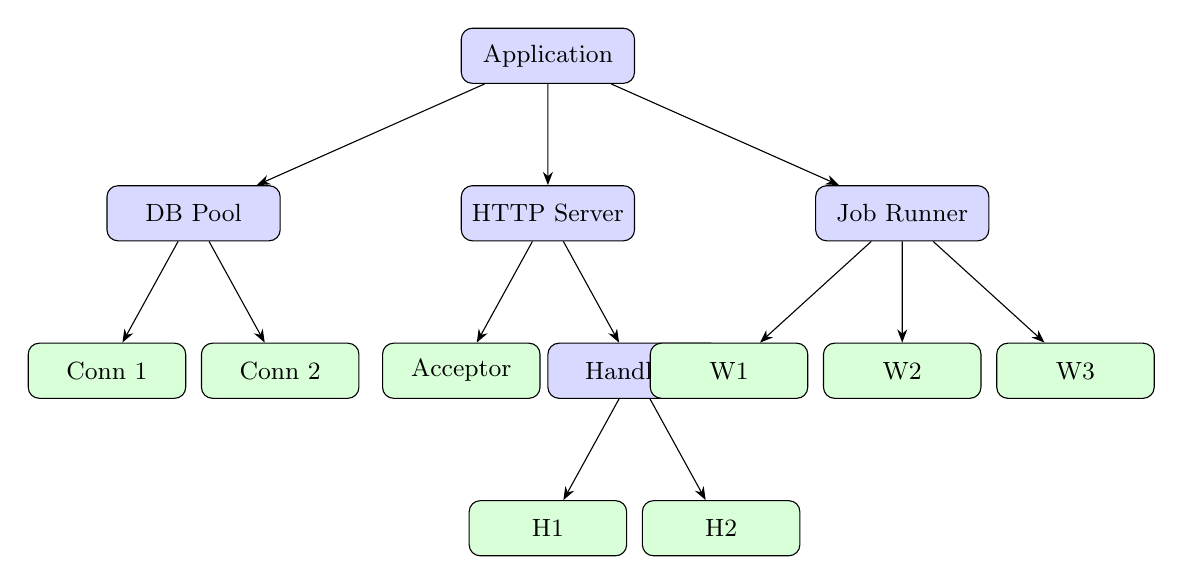
\begin{tikzpicture}[
  level 1/.style={sibling distance=4.5cm, level distance=2cm},
  level 2/.style={sibling distance=2.2cm, level distance=2cm},
  sup/.style={draw, rounded corners, fill=blue!15, minimum width=2.2cm, minimum height=0.7cm, font=\small},
  worker/.style={draw, rounded corners, fill=green!15, minimum width=2cm, minimum height=0.7cm, font=\small},
  edge from parent/.style={draw, -Stealth}
]
\node [sup] {Application}
  child { node [sup] {DB Pool}
    child { node [worker] {Conn 1} }
    child { node [worker] {Conn 2} }
  }
  child { node [sup] {HTTP Server}
    child { node [worker] {Acceptor} }
    child { node [sup] {Handlers}
      child { node [worker] {H1} }
      child { node [worker] {H2} }
    }
  }
  child { node [sup] {Job Runner}
    child { node [worker] {W1} }
    child { node [worker] {W2} }
    child { node [worker] {W3} }
  };
\end{tikzpicture}
\caption{A supervision tree for a typical JAPL web application. Blue nodes are supervisors; green nodes are worker processes. Arrows indicate supervision relationships.}
\label{fig:suptree}
\end{figure}

\subsection{Process Groups and Registries}

Beyond tree-structured supervision, JAPL provides process groups and registries for organizing processes:

\begin{lstlisting}[language=japl,caption={Process groups and registries}]
-- Register a process under a name
Registry.register("cache_server", pid)

-- Look up a process by name
let cache = Registry.lookup("cache_server")

-- Process groups: broadcast to all members
let group = ProcessGroup.new("event_listeners")
ProcessGroup.join(group, listener1)
ProcessGroup.join(group, listener2)
ProcessGroup.broadcast(group, EventOccurred(event_data))
\end{lstlisting}

\subsection{Formal Model of Supervision}

\begin{definition}[Supervision tree]\label{def:suptree}
A supervision tree $\mathcal{T}$ is a rooted tree where:
\begin{itemize}
\item Each internal node is a supervisor $\Sup{s}{\overline{P_i}}$ with strategy $s \in \{\text{OneForOne}, \text{AllForOne}, \text{RestForOne}\}$.
\item Each leaf is a worker process $P$.
\item Each node has restart parameters $(k, t)$ specifying at most $k$ restarts in $t$ seconds.
\end{itemize}
\end{definition}

\begin{definition}[Restart function]\label{def:restart}
The restart function $\mathsf{restart} : \mathsf{Strategy} \times \mathsf{Reason} \times \overline{\Proc} \times \mathbb{N} \to \overline{\Proc} + \mathsf{Escalate}$ is defined by:
\begin{align}
\mathsf{restart}(\text{OneForOne}, r, [P_1, \ldots, P_n], j) &= [P_1, \ldots, P_j^0, \ldots, P_n] \notag \\
\mathsf{restart}(\text{AllForOne}, r, [P_1, \ldots, P_n], j) &= [P_1^0, \ldots, P_n^0] \notag \\
\mathsf{restart}(\text{RestForOne}, r, [P_1, \ldots, P_n], j) &= [P_1, \ldots, P_{j-1}, P_j^0, \ldots, P_n^0] \notag
\end{align}
where $P_i^0$ denotes the initial state of process $P_i$ and $j$ is the index of the failed process. If the restart intensity is exceeded, the function returns $\mathsf{Escalate}$, causing the supervisor itself to fail.
\end{definition}


% ================================================================
% 7. PROCESS LIFECYCLE
% ================================================================
\section{Process Lifecycle}\label{sec:lifecycle}

\subsection{Lifecycle States}

A JAPL process passes through the following states:

\begin{figure}[H]
\centering
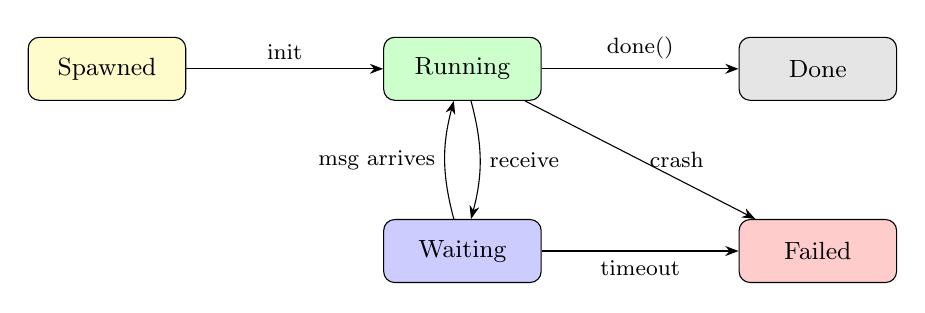
\begin{tikzpicture}[
  state/.style={draw, rounded corners, minimum width=2cm, minimum height=0.8cm, font=\small},
  ->, >=Stealth, auto, node distance=2.5cm
]
\node [state, fill=yellow!20] (spawned) {Spawned};
\node [state, fill=green!20, right=of spawned] (running) {Running};
\node [state, fill=blue!20, below=1.5cm of running] (waiting) {Waiting};
\node [state, fill=gray!20, right=of running] (done) {Done};
\node [state, fill=red!20, below=1.5cm of done] (failed) {Failed};

\path (spawned) edge node {\footnotesize init} (running);
\path (running) edge [bend left=15] node {\footnotesize receive} (waiting);
\path (waiting) edge [bend left=15] node {\footnotesize msg arrives} (running);
\path (running) edge node {\footnotesize done()} (done);
\path (running) edge node [right] {\footnotesize crash} (failed);
\path (waiting) edge node [below] {\footnotesize timeout} (failed);
\end{tikzpicture}
\caption{Process lifecycle state machine.}
\label{fig:lifecycle}
\end{figure}

\subsection{Lifecycle Operations}

The six fundamental process operations are:

\begin{description}
\item[\texttt{spawn}:] Creates a new process. The parent receives a typed $\Pid[A]$ for the new process. The new process begins executing its body function.

\begin{lstlisting}[language=japl,caption={Spawning a process}]
let pid: Pid[WorkerMsg] = Process.spawn(fn -> worker(initial_state))
\end{lstlisting}

\item[\texttt{send}:] Enqueues a typed message in the target process's mailbox. Non-blocking; returns immediately.

\begin{lstlisting}[language=japl,caption={Sending a message}]
Process.send(pid, StartJob(job_id))
\end{lstlisting}

\item[\texttt{receive}:] Blocks the process until a message is available in its mailbox. The received message is pattern-matched.

\begin{lstlisting}[language=japl,caption={Receiving with pattern matching}]
match Process.receive() with
| StartJob(id) -> begin_work(state, id)
| CancelJob(id) -> cancel_work(state, id)
\end{lstlisting}

\item[\texttt{continue}:] A tail-recursive call that advances the process to its next iteration with new state. This is the standard mechanism for process-local state management:

\begin{lstlisting}[language=japl,caption={State evolution through tail recursion}]
fn counter(n: Int) -> Never with Process[CounterMsg] =
  match Process.receive() with
  | Increment -> counter(n + 1)      -- continue with new state
  | Decrement -> counter(n - 1)      -- continue with new state
  | GetCount(reply) ->
      Reply.send(reply, n)
      counter(n)                       -- continue with same state
\end{lstlisting}

\item[\texttt{done}:] Signals successful process termination. The process exits with reason $\mathsf{Normal}$. Transient and temporary child processes are not restarted after normal termination.

\begin{lstlisting}[language=japl,caption={Normal process termination}]
fn one_shot_task(data: TaskData) -> Unit with Process[TaskMsg] =
  let result = compute(data)
  Process.send(data.reply_to, TaskComplete(result))
  done()
\end{lstlisting}

\item[\texttt{fail}:] Signals abnormal process termination with a typed reason. The supervisor is notified and takes action according to its strategy.

\begin{lstlisting}[language=japl,caption={Explicit failure with typed reason}]
fn db_worker(conn: DbConn) -> Never with Process[DbMsg] =
  match Process.receive() with
  | Query(sql, reply) ->
      match Db.execute(conn, sql) with
      | Ok(rows) ->
          Reply.send(reply, Ok(rows))
          db_worker(conn)
      | Err(ConnectionLost(detail)) ->
          fail(DbCrashReason(ConnectionLost(detail)))
\end{lstlisting}
\end{description}

\subsection{Process-Local Tail Recursion as State Management}

A distinctive feature of JAPL's process model (shared with Erlang) is that process-local state is managed through tail recursion rather than mutable variables. The process function takes the current state as a parameter and calls itself with the new state:

\begin{lstlisting}[language=japl,caption={State management via tail recursion}]
type RateLimiterMsg =
  | Request(ClientId, Reply[Bool])
  | ResetBucket(ClientId)
  | GetStats(Reply[RateLimiterStats])

type BucketState = Map[ClientId, { count: Int, reset_at: Timestamp }]

fn rate_limiter(state: BucketState, config: RateLimiterConfig)
    -> Never with Process[RateLimiterMsg] =
  match Process.receive() with
  | Request(client, reply) ->
      let bucket = Map.lookup(state, client)
        |> Option.unwrap_or({ count = 0, reset_at = now() + config.window })
      if bucket.count < config.max_requests then
        Reply.send(reply, True)
        let new_bucket = { bucket | count = bucket.count + 1 }
        rate_limiter(Map.insert(state, client, new_bucket), config)
      else
        Reply.send(reply, False)
        rate_limiter(state, config)
  | ResetBucket(client) ->
      rate_limiter(Map.delete(state, client), config)
  | GetStats(reply) ->
      Reply.send(reply, compute_stats(state))
      rate_limiter(state, config)
\end{lstlisting}

This approach has important advantages over mutable state:

\begin{enumerate}
\item \textbf{No partial updates.} The state transition is atomic: the old state is the parameter, the new state is the argument to the recursive call. There is no window where the state is partially updated.

\item \textbf{State history.} Since state is passed as a value, it is trivial to log, snapshot, or roll back state transitions for debugging or auditing.

\item \textbf{Restart safety.} When a process crashes and is restarted, it begins with fresh, known-good state (the initial parameter). There is no corrupted mutable state to worry about.

\item \textbf{Guaranteed tail-call optimization.} JAPL guarantees tail-call elimination, so process loops consume constant stack space regardless of how many messages they process.
\end{enumerate}


% ================================================================
% 8. COMPARISON
% ================================================================
\section{Comparison with Existing Approaches}\label{sec:comparison}

\Cref{tab:comparison} provides a feature-level comparison of JAPL's process model with the concurrency facilities of Erlang, Go, Akka, Pony, and Gleam.

\begin{table}[H]
\centering
\small
\caption{Comparison of concurrency models across languages.}
\label{tab:comparison}
\begin{tabular}{@{}lcccccc@{}}
\toprule
\textbf{Feature} & \textbf{JAPL} & \textbf{Erlang} & \textbf{Go} & \textbf{Akka} & \textbf{Pony} & \textbf{Gleam} \\
\midrule
Typed messages        & \checkmark & $\times$   & \checkmark & Partial  & \checkmark & \checkmark \\
Process isolation     & \checkmark & \checkmark & $\times$   & $\times$ & \checkmark & \checkmark \\
Supervision trees     & \checkmark & \checkmark & $\times$   & \checkmark & $\times$ & \checkmark \\
Typed supervision     & \checkmark & $\times$   & $\times$   & Partial  & $\times$ & $\times$ \\
Session types         & \checkmark & $\times$   & $\times$   & $\times$ & $\times$ & $\times$ \\
Effect tracking       & \checkmark & $\times$   & $\times$   & $\times$ & $\times$ & $\times$ \\
Location transparency & \checkmark & \checkmark & $\times$   & \checkmark & $\times$ & \checkmark \\
Hot code upgrade      & Planned    & \checkmark & $\times$   & $\times$ & $\times$ & \checkmark \\
Per-process GC        & \checkmark & \checkmark & $\times$   & $\times$ & \checkmark & \checkmark \\
Linear resources      & \checkmark & $\times$   & $\times$   & $\times$ & \checkmark & $\times$ \\
\bottomrule
\end{tabular}
\end{table}

\paragraph{Note on hot code upgrade.} The ``Planned'' status for hot code upgrade in JAPL reflects a deliberate design tension. Erlang and Gleam support hot code swapping via the BEAM's module-loading infrastructure, which benefits from dynamic typing: a new module version can accept messages of any shape, and the programmer is responsible for handling both old- and new-format messages during the transition. In a statically typed language like JAPL, hot-swapping is \emph{harder} because type versioning must be addressed: if version $n$ of a process expects $\mathsf{Msg}_n$ and version $n{+}1$ expects $\mathsf{Msg}_{n+1}$, the runtime must ensure that in-flight messages of type $\mathsf{Msg}_n$ are either drained before the upgrade or translated to $\mathsf{Msg}_{n+1}$ via a compiler-generated migration function. Conversely, static typing makes hot-swapping \emph{safer}: the compiler can verify that the migration function is total and type-correct, that the new process state type is compatible with the serialized state of the old version, and that all callers holding a $\Pid[\mathsf{Msg}_n]$ are updated or provided with a typed adapter. JAPL's planned approach requires each hot-upgradeable module to declare a $\mathsf{Migration}[V_{\text{old}}, V_{\text{new}}]$ instance, providing compile-time assurance that upgrades preserve type safety---a guarantee that neither Erlang nor Gleam can offer.

\subsection{Erlang/OTP}

Erlang is the direct inspiration for JAPL's process model, and JAPL inherits its core insights: lightweight processes, process isolation, asynchronous message passing, supervision trees, and the ``let it crash'' philosophy. The key differences are:

\begin{description}
\item[Static typing.] JAPL's typed mailboxes catch message-protocol errors at compile time. Erlang's Dialyzer provides success typing but cannot enforce exhaustive message handling or session-type compliance.

\item[Typed crash reasons.] In Erlang, crash reasons are arbitrary terms. In JAPL, they are typed algebraic data types, enabling pattern-matching on failure modes in supervision logic.

\item[Effect tracking.] JAPL's effect system makes concurrency operations visible in function signatures. In Erlang, any function can send messages or spawn processes, and this is not reflected in the function's type.

\item[Ownership for resources.] Erlang relies on GC for all memory management. JAPL's linear types provide deterministic resource cleanup and safe ownership transfer between processes.
\end{description}

Erlang's advantages over JAPL include its mature ecosystem, battle-tested runtime (the BEAM), hot code reloading, and three decades of production experience. JAPL aims to preserve Erlang's strengths while adding the benefits of static typing.

\subsection{Go}

Go's goroutines and channels provide syntactically lightweight concurrency, but the model differs from JAPL's in fundamental ways:

\begin{description}
\item[Shared memory.] Go goroutines share the process memory space. While channels provide a communication mechanism, nothing prevents goroutines from accessing shared variables, and data races are a common source of bugs. Go's race detector is dynamic, not static.

\item[No supervision.] Go has no built-in supervision mechanism. A panicking goroutine crashes the program unless explicitly recovered. Building supervision in Go requires manual bookkeeping.

\item[Channel typing.] Go channels are typed, which is a strength. However, channels are point-to-point, and there is no equivalent of Erlang/JAPL's selective receive or mailbox semantics. Complex protocols require careful channel management.

\item[Goroutine leaks.] Since goroutines are not supervised, a goroutine that blocks on a channel read forever is a resource leak. Detecting and preventing goroutine leaks requires discipline and tooling external to the language.
\end{description}

Go's advantages include its simplicity, fast compilation, excellent tooling, and large ecosystem. JAPL draws inspiration from Go's pragmatic approach to tooling and compilation speed.

\subsection{Akka}

Akka provides actor-based concurrency on the JVM, with supervision trees and location transparency. The comparison with JAPL:

\begin{description}
\item[JVM overhead.] Akka actors share the JVM heap and can access each other's state through Java references, bypassing the actor abstraction. JAPL enforces isolation at the language level.

\item[Akka Typed.] Akka Typed addresses some message-typing concerns but operates within Java's type system, which lacks algebraic data types and effect tracking. Protocol violations can still occur through type erasure and runtime casts.

\item[Complexity.] The Akka API surface is large, with many ways to accomplish the same task. JAPL aims for a smaller, more principled set of primitives.

\item[Library vs.\ language.] Supervision in Akka is a library feature. In JAPL, it is a language feature with syntactic support (the \texttt{supervisor} declaration) and type-system integration.
\end{description}

\subsection{Pony}

Pony's reference capabilities provide a novel approach to actor safety:

\begin{description}
\item[Reference capabilities.] Pony uses a capability system (iso, val, ref, box, tag, trn) to prevent data races. This is theoretically elegant but imposes significant cognitive burden.

\item[No supervision.] Pony does not provide built-in supervision trees. Error handling is left to the programmer.

\item[Actor isolation.] Pony achieves actor isolation through its capability system rather than per-actor heaps. This allows zero-copy message passing for data with appropriate capabilities, but requires understanding the capability system.
\end{description}

JAPL takes a different approach: isolation through per-process heaps and ownership types, which is conceptually simpler (immutable data is shared freely; mutable resources have single owners) while achieving similar safety guarantees.

\subsection{Gleam}

Gleam compiles to BEAM bytecode and provides static typing for the Erlang ecosystem:

\begin{description}
\item[Shared runtime.] Gleam inherits BEAM's runtime characteristics (per-process heaps, preemptive scheduling, supervision) and can interoperate with Erlang and Elixir libraries.

\item[Type system scope.] Gleam's type system is simpler than JAPL's: it lacks effect tracking, session types, linear types, and capability types. This makes Gleam more accessible but provides fewer static guarantees.

\item[Interoperability.] Gleam's BEAM compatibility is a significant practical advantage. JAPL targets its own runtime, which provides more control but requires building an ecosystem from scratch.
\end{description}


% ================================================================
% 9. IMPLEMENTATION
% ================================================================
\section{Implementation}\label{sec:implementation}

This section describes the key implementation techniques for JAPL's process runtime, targeting scalability to millions of concurrent processes on commodity hardware.

\subsection{Lightweight Process Representation}

Each JAPL process is represented as a lightweight structure containing:

\begin{itemize}
\item A \textbf{process control block} (PCB): status flags, priority, reduction counter, mailbox pointer, links/monitors list, supervisor reference.
\item A \textbf{private heap}: a small, separately collected memory region for the process's local data. Initial size is 2\,KB, growing as needed.
\item A \textbf{stack}: for the process's continuation. Since JAPL guarantees tail-call elimination for process loops, the stack remains small.
\item A \textbf{mailbox}: a queue of incoming messages (described in \Cref{sec:impl-mailbox}).
\end{itemize}

The total overhead per idle process is approximately 4--8\,KB, enabling millions of processes per node on machines with tens of gigabytes of RAM.

\subsection{Scheduler Design}

JAPL's scheduler follows the Erlang BEAM model with enhancements:

\begin{description}
\item[Scheduler threads.] The runtime creates one scheduler thread per CPU core. Each scheduler thread has a run queue of processes ready to execute.

\item[Preemptive scheduling.] Each process is assigned a \emph{reduction budget} (e.g., 4000 reductions). Function calls, message sends, and receives each consume one or more reductions. When a process exhausts its budget, it is preempted and placed at the back of its scheduler's run queue.

\item[Work stealing.] When a scheduler's run queue is empty, it attempts to steal processes from other schedulers' queues. This provides automatic load balancing across cores.

\item[Priority queues.] Each scheduler maintains multiple priority levels (high, normal, low). High-priority processes (e.g., supervisors, timers) are scheduled preferentially.

\item[Priority inversion avoidance.] In shared-memory systems, priority inversion occurs when a low-priority thread holds a lock needed by a high-priority thread. JAPL's process model avoids this pathology structurally: since processes do not share memory or locks, the classical Coffman-style priority inversion cannot arise. However, a \emph{message-level} analog exists: a high-priority process may send a request (via $\mathsf{Reply}[T]$) to a low-priority process and block on the reply. If the low-priority process is starved of scheduler time, the high-priority process is effectively delayed. JAPL addresses this through \emph{priority inheritance on reply channels}: when a high-priority process blocks on a $\mathsf{Reply.await}$, the runtime temporarily elevates the priority of the target process to match the waiter's priority. This elevation persists until the reply is sent, at which point the target process reverts to its original priority. During work stealing, stolen processes retain their (possibly elevated) priority, ensuring that a process promoted due to a pending reply is not demoted simply by being migrated to a different scheduler's queue. This mechanism ensures that priority queues and work stealing interact correctly without reintroducing the priority inversion problem.
\end{description}

\begin{figure}[H]
\centering
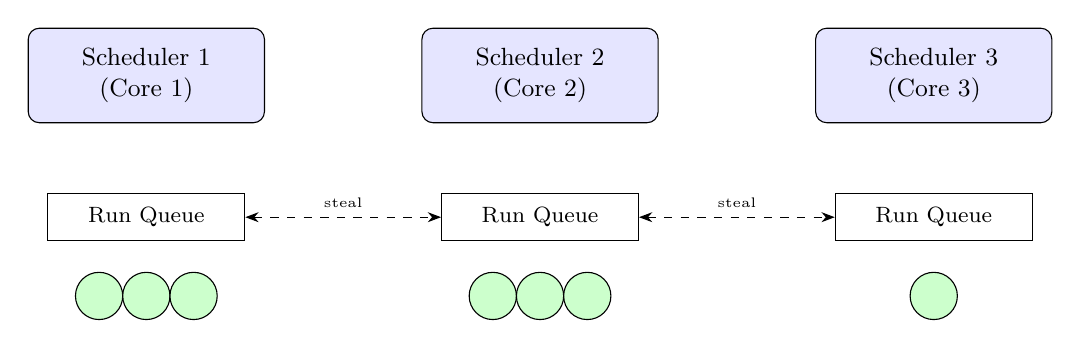
\begin{tikzpicture}[
  sched/.style={draw, rounded corners, fill=blue!10, minimum width=3cm, minimum height=1.2cm, font=\small},
  queue/.style={draw, minimum width=2.5cm, minimum height=0.6cm, font=\footnotesize},
  proc/.style={draw, circle, fill=green!20, minimum size=0.6cm, font=\tiny},
  ->, >=Stealth
]
\node [sched, align=center] (s1) at (0,0) {Scheduler 1\\(Core 1)};
\node [sched, align=center] (s2) at (5,0) {Scheduler 2\\(Core 2)};
\node [sched, align=center] (s3) at (10,0) {Scheduler 3\\(Core 3)};

\node [queue] (q1) at (0,-1.8) {Run Queue};
\node [queue] (q2) at (5,-1.8) {Run Queue};
\node [queue] (q3) at (10,-1.8) {Run Queue};

\foreach \x in {-0.6,0,0.6} {
  \node [proc] at (\x, -2.8) {};
}
\foreach \x in {4.4,5,5.6} {
  \node [proc] at (\x, -2.8) {};
}
\node [proc] at (10, -2.8) {};

\draw [dashed, <->] (q2) -- node [above, font=\tiny] {steal} (q3);
\draw [dashed, <->] (q1) -- node [above, font=\tiny] {steal} (q2);
\end{tikzpicture}
\caption{Work-stealing scheduler architecture. Each core has a scheduler with its own run queue. Idle schedulers steal work from busy ones.}
\label{fig:scheduler}
\end{figure}

\subsection{Mailbox Data Structures}\label{sec:impl-mailbox}

The mailbox is a critical data structure, as every inter-process communication passes through it. JAPL's mailbox implementation has two components:

\begin{description}
\item[Message queue.] A lock-free, multi-producer, single-consumer (MPSC) queue. Multiple processes can send messages concurrently without contention (each sender appends to the queue via a CAS operation on the tail pointer). The owning process is the sole consumer, so receives require no synchronization.

\item[Selective receive index.] For processes that use selective receive, the mailbox maintains an auxiliary index that maps message constructors (tags) to positions in the queue. This enables $O(1)$ lookup for selective receive by tag, avoiding the $O(n)$ scan that Erlang's selective receive requires.
\end{description}

\begin{lstlisting}[language=japl,caption={Selective receive with efficient tag-based lookup}]
-- Without selective receive: messages processed in order
fn simple_worker(state: State) -> Never with Process[WorkerMsg] =
  match Process.receive() with
  | msg -> handle(state, msg)

-- With selective receive: priority messages handled first
fn priority_worker(state: State) -> Never with Process[WorkerMsg] =
  -- Efficiently finds the first Priority message in the mailbox
  match Process.receive_matching(fn m -> is_priority(m)) with
  | Some(Priority(data)) -> handle_priority(state, data)
  | None ->
      -- No priority messages; handle the next regular message
      match Process.receive() with
      | msg -> handle(state, msg)
\end{lstlisting}

\subsection{Process Isolation Guarantees}

JAPL's runtime enforces process isolation through multiple mechanisms:

\begin{enumerate}
\item \textbf{Per-process heaps.} Each process allocates memory from its own heap region. References between heaps are forbidden for mutable data.

\item \textbf{Immutable data sharing.} Immutable values (which constitute the vast majority of data in functional programs) can be shared across process heaps via pointer sharing, since concurrent reads of immutable data are safe. The GC handles reachability tracking.

\item \textbf{Message copying for small messages.} Small messages (below a configurable threshold, default 64 bytes) are copied into the receiving process's heap. This avoids cross-heap references for small messages and improves cache locality.

\item \textbf{Reference counting for large immutable messages.} Large immutable messages (strings, byte arrays, large records) are allocated in a shared immutable heap and reference-counted. Since they are immutable, concurrent reference counting is safe.

\item \textbf{Ownership transfer for mutable resources.} Mutable resources are moved (not copied) between processes. The runtime ensures that after a move, the sending process's reference is invalidated.
\end{enumerate}

\subsection{Green Threads vs.\ OS Threads}

JAPL processes are green threads (user-space threads managed by the runtime) rather than OS threads. The comparison:

\begin{table}[H]
\centering
\small
\caption{Green threads vs.\ OS threads.}
\label{tab:threads}
\begin{tabular}{@{}lll@{}}
\toprule
\textbf{Property} & \textbf{Green Threads (JAPL)} & \textbf{OS Threads} \\
\midrule
Creation cost        & $\sim$2--8 KB memory            & $\sim$1--8 MB stack \\
Context switch       & $\sim$100 ns (user-space)       & $\sim$1--10 $\mu$s (kernel) \\
Max concurrent       & Millions per node               & Thousands per node \\
Scheduling           & Runtime (cooperative/preemptive) & OS kernel \\
Isolation            & Per-process heap (JAPL runtime)  & Shared process memory \\
Blocking I/O         & Handled by I/O scheduler        & Blocks OS thread \\
\bottomrule
\end{tabular}
\end{table}

The JAPL runtime includes a dedicated I/O scheduler that offloads blocking operations (file I/O, DNS resolution, long-running FFI calls) to a pool of OS threads, ensuring that blocking I/O does not stall the green thread scheduler.

\subsection{Garbage Collection}

JAPL uses a hybrid GC strategy:

\begin{description}
\item[Per-process generational GC.] Each process's private heap has a two-generation collector. Young generation collection is triggered frequently (every few hundred reductions) and is very fast (typically microseconds) because process heaps are small. Old generation collection is less frequent.

\item[Process death reclamation.] When a process terminates, its entire heap is freed in one operation, with no need for GC. In systems with many short-lived processes, this provides excellent throughput.

\item[Shared immutable heap.] Large immutable values shared across processes live in a separate heap with concurrent mark-sweep collection. Since this data is immutable, no write barriers are needed, simplifying the collector significantly.
\end{description}


% ================================================================
% 10. FORMAL PROPERTIES
% ================================================================
\section{Formal Properties}\label{sec:properties}

\subsection{Typed Message Safety}

\begin{theorem}[Type preservation]\label{thm:preservation}
If $\Gamma \vdash P$ and $P \rightarrow P'$, then $\Gamma' \vdash P'$ for some $\Gamma' \supseteq \Gamma$.
\end{theorem}

\begin{proof}
By induction on the derivation of $P \rightarrow P'$.

\textbf{Case R-Comm:} We have $\sendf{x}{v}.P_1 \ppar \recvf{x}{y}.P_2 \rightarrow P_1 \ppar P_2[v/y]$. By T-Send, $\Gamma \vdash v : A$ where $\Gamma(x) = \Pid[A]$. By T-Recv, $\Gamma, y : A \vdash P_2$. By the substitution lemma, $\Gamma \vdash P_2[v/y]$. Since $\Gamma \vdash P_1$ (from the premise of T-Send), we have $\Gamma \vdash P_1 \ppar P_2[v/y]$.

\textbf{Case R-Spawn:} We have $\spawn{x}{A}{P_1}{P_2} \rightarrow \pnew{x : \Pid[A]}(P_1 \ppar P_2)$. By T-Spawn, $\Gamma, x : \Pid[A] \vdash P_1$ and $\Gamma, x : \Pid[A] \vdash P_2$. Let $\Gamma' = \Gamma, x : \Pid[A]$. Then $\Gamma' \vdash P_1 \ppar P_2$ and $\Gamma \vdash \pnew{x : \Pid[A]}(P_1 \ppar P_2)$ by T-New (with $\Gamma' \supseteq \Gamma$).

\textbf{Case R-Fail:} The supervisor applies the restart function, which creates fresh instances of the same process type. By T-Sup, each child specification includes a start function of the appropriate type, so the restarted processes are well-typed.

The remaining cases (R-Match, R-Par, R-New) follow by straightforward induction.
\end{proof}

\begin{corollary}[No message type errors at runtime]\label{cor:no-msg-errors}
In a well-typed JAPL program, a process with mailbox type $A$ never receives a message that is not of type $A$.
\end{corollary}

\subsection{Deadlock Freedom}

Deadlock in process-based systems can arise when processes form a circular wait on message reception. JAPL's supervision model provides a practical (though not absolute) guarantee against deadlock:

\begin{definition}[Supervision-disciplined network]\label{def:supdiscipline}
A process network is \emph{supervision-disciplined} if:
\begin{enumerate}
\item Every process is part of a supervision tree.
\item Communication follows the supervision hierarchy: children send messages to their supervisor (or siblings in the same supervision group), and supervisors send messages to their children.
\item All receive operations have timeouts at supervision boundaries.
\end{enumerate}
\end{definition}

\begin{theorem}[Deadlock freedom under supervision discipline]\label{thm:deadlock-free}
A supervision-disciplined process network is deadlock-free.
\end{theorem}

\begin{proof}
Assume for contradiction that a deadlock exists: a cycle $P_1 \to P_2 \to \cdots \to P_k \to P_1$ where each $P_i$ is waiting for a message from $P_{i+1}$ (indices mod $k$).

By the supervision discipline, communication follows the supervision hierarchy. The supervision tree is acyclic (it is a tree). Therefore, the communication graph is a subgraph of the tree, augmented with sibling edges. In either case, a cycle would require an edge from a descendant to an ancestor, which the discipline forbids for blocking communication.

If any $P_i$ uses a timed receive at a supervision boundary, the timeout will fire, breaking the potential deadlock by causing $P_i$ to take an alternative action (fail, retry, or escalate to its supervisor).
\end{proof}

\begin{remark}
The supervision discipline is sufficient but not always necessary. Many practical process networks that violate the discipline are still deadlock-free. However, the discipline provides a compositional, statically checkable criterion.
\end{remark}

\subsubsection{Lateral Communication and Deadlock Detection}

We acknowledge that the supervision-disciplined network assumption is restrictive. In real-world actor systems, \emph{lateral communication}---messages between sibling processes, unrelated process groups, or processes discovered via a Registry---is common and often necessary. Registry-based communication (e.g., \texttt{Registry.lookup("service\_name")}) introduces edges in the communication graph that do not follow the supervision hierarchy, potentially creating cycles that violate the tree-structured assumption of \Cref{thm:deadlock-free}.

JAPL adopts a two-tier strategy to handle this. For \emph{tree-structured communication} (parent--child and sibling messages within a supervision group), the deadlock prevention guarantee of \Cref{thm:deadlock-free} applies statically. For \emph{lateral communication} that escapes the supervision hierarchy, JAPL provides a \emph{deadlock detection} effect:

\begin{lstlisting}[language=japl,caption={Deadlock-aware lateral communication}]
-- Lateral send with deadlock detection enabled
fn request_from_peer(peer: Pid[PeerMsg], data: RequestData)
    -> Result[Response, Timeout] with Process =
  let reply = Reply.new()
  Process.send(peer, PeerRequest(data, reply))
  -- Timed await: breaks potential deadlock cycles
  Reply.await_timeout(reply, 5000)
\end{lstlisting}

The runtime maintains a lightweight \emph{wait-for graph} over processes that are blocked on $\mathsf{Reply.await}$ or $\mathsf{receive}$ calls involving lateral channels. When a cycle is detected in this graph, the runtime delivers a $\mathsf{DeadlockDetected}$ signal to the youngest process in the cycle (by process creation time), causing it to fail and be restarted by its supervisor. This hybrid approach---static prevention for hierarchical communication, dynamic detection for lateral communication---preserves the strong guarantees of the supervision discipline where they apply while permitting the flexible communication topologies that practical systems require.

\subsection{Progress Guarantees}

\begin{definition}[Progress]\label{def:progress}
A well-typed process $P$ with mailbox type $A$ \emph{makes progress} if it is either:
\begin{enumerate}
\item Able to perform an internal reduction ($P \rightarrow P'$), or
\item Waiting to receive a message and able to accept any message of type $A$, or
\item Successfully terminated ($P = \donef$), or
\item Failed and being handled by its supervisor.
\end{enumerate}
\end{definition}

\begin{theorem}[Progress for well-typed processes]\label{thm:progress}
If $\Gamma \vdash P$ and $P \neq \donef$ and $P$ is not waiting for a message, then there exists $P'$ such that $P \rightarrow P'$.
\end{theorem}

\begin{proof}
By induction on the typing derivation of $P$.

\textbf{Case T-Send:} $P = \sendf{x}{v}.P'$. If there exists a process $Q = \recvf{x}{y}.Q'$ in parallel, then R-Comm applies. If not, the send is asynchronous: the message is enqueued and $P$ transitions to $P'$.

\textbf{Case T-Match:} $P = \mathsf{match}\; v\; \{\overline{p_i \Rightarrow P_i}\}$. Since the typing rule requires exhaustive pattern matching over all constructors of the message type $A$, there exists some $j$ such that $p_j$ matches $v$, and R-Match applies.

\textbf{Case T-Spawn:} R-Spawn applies immediately.

\textbf{Case T-Sup:} The supervisor monitors its children. If any child has failed, R-Fail applies. Otherwise, the supervisor itself is waiting for a child event (a form of receive).
\end{proof}

\subsection{Typed Reply Safety}

\begin{theorem}[Reply linearity]\label{thm:reply-linearity}
If $\Gamma \vdash P$ and $P$ contains a binding $r : \mathsf{Reply}[T]$, then $r$ is used exactly once in $P$: exactly one $\mathsf{Reply.send}(r, v)$ occurs on every execution path through $P$.
\end{theorem}

\begin{proof}
The $\mathsf{Reply}[T]$ type is linear. JAPL's linear type checker ensures that every linear value is consumed exactly once. If $r$ is unused on some path, the checker reports a ``linear value not consumed'' error. If $r$ is used twice, the checker reports a ``linear value used after consumption'' error. Since the program is well-typed, neither case applies.
\end{proof}


% ================================================================
% 11. DISCUSSION
% ================================================================
\section{Discussion}\label{sec:discussion}

\subsection{When Processes Are Overkill}

Not every concurrent task warrants a process. For fine-grained data parallelism---mapping a function over a large array, parallel sorting, matrix operations---the overhead of process creation and message passing is unnecessary. JAPL addresses this through two mechanisms:

\begin{description}
\item[Parallel combinators.] Functions like $\mathsf{List.par\_map}$ and $\mathsf{Array.par\_fold}$ provide data-parallel operations that use the scheduler's thread pool directly, without creating processes. These are implemented as work-stealing parallel loops at the runtime level.

\begin{lstlisting}[language=japl,caption={Data parallelism without processes}]
-- Parallel map: uses scheduler threads, not processes
let results = List.par_map(large_list, fn item ->
  expensive_computation(item)
)

-- Sequential map: single-threaded
let results = List.map(large_list, fn item ->
  expensive_computation(item)
)
\end{lstlisting}

\item[Structured concurrency scopes.] For medium-grained parallelism (e.g., making several API calls concurrently), JAPL provides structured concurrency within a lexical scope:

\begin{lstlisting}[language=japl,caption={Structured concurrency scope}]
fn fetch_dashboard_data(user_id: UserId) -> DashboardData
    with Io, Net =
  -- All three fetches run concurrently; scope waits for all
  let (profile, orders, notifications) = concurrent {
    fetch_profile(user_id),
    fetch_orders(user_id),
    fetch_notifications(user_id),
  }
  { profile, orders, notifications }
\end{lstlisting}
\end{description}

\subsection{Integration with the Effect System}

The $\mathsf{Process}[A]$ effect interacts with other effects in JAPL's effect system:

\begin{description}
\item[Effect subsumption.] $\mathsf{Process}[A]$ subsumes $\mathsf{Async}$: any asynchronous operation can be expressed as a process operation. The reverse is not true: $\mathsf{Async}$ does not imply the ability to spawn processes or receive typed messages.

\item[Effect handlers at process boundaries.] When spawning a process, the parent provides effect handlers for the child's effects. For example, a child process that performs $\mathsf{Io}$ has its I/O routed through the runtime's I/O scheduler. This is transparent to the child.

\item[Pure process logic.] The body of a process loop often calls pure functions for business logic, using processes only for state management and message routing. The effect system makes this separation explicit: pure helper functions have no effects in their signatures.
\end{description}

\subsection{Distribution Considerations}

JAPL's location-transparent PIDs enable distribution, but introduce challenges:

\begin{description}
\item[Serialization.] Messages sent to remote processes must be serialized. JAPL uses type-derived serialization: any type with a $\mathsf{Serialize}$ trait implementation can cross node boundaries. Types that cannot be serialized (e.g., those containing function closures or mutable resources) cause a compile-time error if used in a context that requires distribution.

\item[Partial failure.] Network partitions can cause message loss and process unreachability. JAPL's monitoring system detects node disconnections and delivers $\mathsf{NodeDown}$ messages to processes that monitor remote nodes.

\item[Consistency.] JAPL does not impose a global consistency model. Processes on different nodes communicate via asynchronous messages, and any consistency guarantees must be built at the application level (e.g., using consensus protocols). The supervision tree model naturally supports the ``let it crash and retry'' approach to network failures.
\end{description}

\subsection{Performance Considerations}

The process-based model introduces overhead compared to shared-memory concurrency:

\begin{description}
\item[Message copying.] While immutable data can be shared by reference, crossing process boundaries for mutable data requires copying or ownership transfer. For most applications, the cost is negligible; for high-throughput data pipelines, ownership transfer (zero-copy) is available.

\item[Context switching.] Green thread context switches ($\sim$100\,ns) are much cheaper than OS thread context switches ($\sim$1--10\,$\mu$s) but more expensive than atomic operations ($\sim$10--50\,ns). For contended data structures accessed billions of times, lock-free shared memory would be faster. JAPL's position is that such scenarios are rare and can be addressed with the parallel combinator escape hatch.

\item[Memory overhead.] Per-process heaps provide isolation but increase memory usage compared to a shared heap. The minimum overhead (4--8\,KB per process) is acceptable for most applications but may be significant for systems with tens of millions of processes.
\end{description}

\subsection{Limitations and Future Work}

Several aspects of JAPL's process model are active areas of research and development:

\begin{enumerate}
\item \textbf{Multiparty session types.} The current session type support handles two-party sessions. Extending to multiparty session types~\citep{honda2008multiparty} would enable verification of complex distributed protocols involving multiple participants.

\item \textbf{Hot code upgrade.} Erlang supports hot code swapping---updating running code without stopping the system. JAPL plans to support this through typed module versioning, where the type system ensures that upgraded code is compatible with existing process states.

\item \textbf{Process algebra tooling.} We plan to develop tools that extract process algebra models from JAPL code and verify properties (deadlock freedom, protocol compliance) using model checking techniques.

\item \textbf{Hardware acceleration.} For some workloads, mapping processes to hardware threads (via OS threads or SIMD lanes) could provide significant speedups. We are investigating hybrid scheduling strategies.

\item \textbf{Formal verification.} Integrating with proof assistants (Coq, Lean) to provide machine-checked proofs of process protocol correctness is a long-term goal.
\end{enumerate}


% ================================================================
% 12. CONCLUSION
% ================================================================
\section{Conclusion}\label{sec:conclusion}

We have presented JAPL's process-based concurrency model, which rejects shared-memory concurrency in favor of isolated, lightweight processes communicating through typed mailboxes under hierarchical supervision. This design, rooted in the Erlang/OTP tradition and extended with modern type theory, provides several advantages over both shared-memory and untyped actor systems:

\begin{enumerate}
\item \textbf{Data race freedom by construction.} Process isolation eliminates data races without requiring locks, atomics, or complex memory models.

\item \textbf{Typed message safety.} Typed mailboxes prevent message-protocol errors at compile time, catching a large class of bugs that are silent in dynamically-typed actor systems.

\item \textbf{Compositional fault tolerance.} Supervision trees, integrated into the type system with typed crash reasons and declarative backoff, provide hierarchical fault domains that compose naturally.

\item \textbf{Effect-tracked concurrency.} The $\mathsf{Process}$ effect makes concurrency visible in function signatures, enabling clean separation of pure logic from concurrent state management.

\item \textbf{Formal foundations.} The categorical semantics (presheaf categories over time, profunctors for communication) and typed $\pi$-calculus provide rigorous foundations for reasoning about process behavior, with proofs of type preservation, progress, and deadlock freedom under supervision discipline.
\end{enumerate}

The process-based model is not without tradeoffs: it introduces overhead for fine-grained parallelism, requires explicit message passing for communication, and adds complexity for distribution. JAPL addresses these through parallel combinators, structured concurrency scopes, and location-transparent PIDs respectively.

Ultimately, JAPL's thesis is that \emph{the shared-memory model is the wrong default for concurrent programming}. Shared memory makes the common case (independent concurrent tasks) unnecessarily dangerous and the hard case (coordinated concurrent tasks) nearly intractable. Process isolation makes the common case safe by default and the hard case manageable through typed protocols and supervision. Three decades of Erlang/OTP's success in telecommunications, along with the growing adoption of actor-based systems in distributed computing, provide strong empirical support for this thesis. JAPL's contribution is to bring the full power of modern type theory to bear on this proven model.

\vspace{1em}
\noindent
\textit{``Pure functions handle logic, supervised processes handle time and failure, and ownership handles resources.''}


% ================================================================
% REFERENCES
% ================================================================
\bibliographystyle{plainnat}

\begin{thebibliography}{40}

\bibitem[Agha(1986)]{agha1986actors}
Gul~A. Agha.
\newblock \emph{Actors: A Model of Concurrent Computation in Distributed Systems}.
\newblock MIT Press, 1986.

\bibitem[Armstrong(2003)]{armstrong2003making}
Joe Armstrong.
\newblock Making reliable distributed systems in the presence of software errors.
\newblock PhD thesis, Royal Institute of Technology, Stockholm, 2003.

\bibitem[Armstrong(2007)]{armstrong2007programming}
Joe Armstrong.
\newblock \emph{Programming Erlang: Software for a Concurrent World}.
\newblock Pragmatic Bookshelf, 2007.

\bibitem[Boehm and Adve(2008)]{boehm2008foundations}
Hans-J. Boehm and Sarita~V. Adve.
\newblock Foundations of the {C}++ concurrency memory model.
\newblock In \emph{PLDI}, pages 68--78. ACM, 2008.

\bibitem[Caires and Pfenning(2010)]{caires2010session}
Lu{\'\i}s Caires and Frank Pfenning.
\newblock Session types as intuitionistic linear propositions.
\newblock In \emph{CONCUR}, volume 6269 of \emph{LNCS}, pages 222--236. Springer, 2010.

\bibitem[Cattani and Winskel(1997)]{cattani1997presheaf}
Gian~Luca Cattani and Glynn Winskel.
\newblock Presheaf models for concurrency.
\newblock In \emph{CSL}, volume 1414 of \emph{LNCS}, pages 58--75. Springer, 1997.

\bibitem[Clebsch et~al.(2015)]{clebsch2015deny}
Sylvan Clebsch, Sophia Drossopoulou, Sebastian Blessing, and Andy McNeil.
\newblock Deny capabilities for safe, fast actors.
\newblock In \emph{AGERE!}, pages 1--12. ACM, 2015.

\bibitem[Coffman et~al.(1971)]{coffman1971system}
Edward~G. Coffman, Michael~J. Elphick, and Arie Shoshani.
\newblock System deadlocks.
\newblock \emph{ACM Computing Surveys}, 3(2):67--78, 1971.

\bibitem[Donovan and Kernighan(2015)]{donovan2015go}
Alan~A.A. Donovan and Brian~W. Kernighan.
\newblock \emph{The Go Programming Language}.
\newblock Addison-Wesley, 2015.

\bibitem[Gleam(2023)]{gleam2023}
{Gleam Team}.
\newblock The {Gleam} programming language.
\newblock \url{https://gleam.run}, 2023.

\bibitem[Hewitt et~al.(1973)]{hewitt1973universal}
Carl Hewitt, Peter Bishop, and Richard Steiger.
\newblock A universal modular {ACTOR} formalism for artificial intelligence.
\newblock In \emph{IJCAI}, pages 235--245, 1973.

\bibitem[Hoare(1978)]{hoare1978communicating}
C.~A.~R. Hoare.
\newblock Communicating sequential processes.
\newblock \emph{Communications of the ACM}, 21(8):666--677, 1978.

\bibitem[Honda(1993)]{honda1993types}
Kohei Honda.
\newblock Types for dyadic interaction.
\newblock In \emph{CONCUR}, volume 715 of \emph{LNCS}, pages 509--523. Springer, 1993.

\bibitem[Honda et~al.(1998)]{honda1998language}
Kohei Honda, Vasco~T. Vasconcelos, and Makoto Kubo.
\newblock Language primitives and type discipline for structured communication-based programming.
\newblock In \emph{ESOP}, volume 1381 of \emph{LNCS}, pages 122--138. Springer, 1998.

\bibitem[Honda et~al.(2008)]{honda2008multiparty}
Kohei Honda, Nobuko Yoshida, and Marco Carbone.
\newblock Multiparty asynchronous session types.
\newblock In \emph{POPL}, pages 273--284. ACM, 2008.

\bibitem[Joyal et~al.(1996)]{joyal1996bisimulation}
Andr{\'e} Joyal, Mogens Nielsen, and Glynn Winskel.
\newblock Bisimulation from open maps.
\newblock \emph{Information and Computation}, 127(2):164--185, 1996.

\bibitem[Lightbend(2023)]{lightbend2023akka}
{Lightbend}.
\newblock {Akka}: Build concurrent, distributed, and resilient message-driven applications.
\newblock \url{https://akka.io}, 2023.

\bibitem[Lindahl and Sagonas(2006)]{lindahl2006practical}
Tobias Lindahl and Konstantinos Sagonas.
\newblock Practical type inference based on success typings.
\newblock In \emph{PPDP}, pages 167--178. ACM, 2006.

\bibitem[Manson et~al.(2005)]{manson2005java}
Jeremy Manson, William Pugh, and Sarita~V. Adve.
\newblock The {Java} memory model.
\newblock In \emph{POPL}, pages 378--391. ACM, 2005.

\bibitem[Michael(2004)]{michael2004hazard}
Maged~M. Michael.
\newblock Hazard pointers: Safe memory reclamation for lock-free objects.
\newblock \emph{IEEE Transactions on Parallel and Distributed Systems}, 15(6):491--504, 2004.

\bibitem[Miller(2006)]{miller2006robust}
Mark~S. Miller.
\newblock \emph{Robust Composition: Towards a Unified Approach to Access Control and Concurrency Control}.
\newblock PhD thesis, Johns Hopkins University, 2006.

\bibitem[Milner(1980)]{milner1980calculus}
Robin Milner.
\newblock \emph{A Calculus of Communicating Systems}.
\newblock Springer, 1980.

\bibitem[Milner(1992)]{milner1992calculus}
Robin Milner, Joachim Parrow, and David Walker.
\newblock A calculus of mobile processes, {I} and {II}.
\newblock \emph{Information and Computation}, 100(1):1--77, 1992.

\bibitem[Milner(1999)]{milner1999communicating}
Robin Milner.
\newblock \emph{Communicating and Mobile Systems: the $\pi$-Calculus}.
\newblock Cambridge University Press, 1999.

\bibitem[Pike(2012)]{pike2012concurrency}
Rob Pike.
\newblock Concurrency is not parallelism.
\newblock Talk at Heroku's Waza conference, 2012.
\newblock \url{https://go.dev/blog/waza-talk}.

\bibitem[Reeves(1997)]{reeves1997mars}
Glenn~E. Reeves.
\newblock What really happened on {Mars}?
\newblock \url{https://www.cs.cornell.edu/courses/cs614/1999sp/papers/pathfinder.html}, 1997.

\bibitem[Roestenburg et~al.(2016)]{roestenburg2016akka}
Raymond Roestenburg, Rob Bakker, and Rob Williams.
\newblock \emph{Akka in Action}.
\newblock Manning Publications, 2016.

\bibitem[Roscoe(1998)]{roscoe1998theory}
A.~W. Roscoe.
\newblock \emph{The Theory and Practice of Concurrency}.
\newblock Prentice Hall, 1998.

\bibitem[Serebryany and Iskhodzhanov(2012)]{serebryany2012threadsanitizer}
Konstantin Serebryany and Timur Iskhodzhanov.
\newblock {ThreadSanitizer}: data race detection in practice.
\newblock In \emph{WBIA}, pages 62--71. ACM, 2012.

\bibitem[Sewell et~al.(2010)]{sewell2010x86}
Peter Sewell, Susmit Sarkar, Scott Owens, Francesco~Zappa Nardelli, and Magnus~O. Myreen.
\newblock x86-{TSO}: A rigorous and usable programmer's model for x86 multiprocessors.
\newblock \emph{Communications of the ACM}, 53(7):89--97, 2010.

\bibitem[Vasconcelos(1998)]{vasconcelos1998language}
Vasco~T. Vasconcelos.
\newblock Language primitives and type discipline for structured communication-based programming.
\newblock PhD thesis, Keio University, 1998.

\bibitem[Wadler(2012)]{wadler2012propositions}
Philip Wadler.
\newblock Propositions as sessions.
\newblock In \emph{ICFP}, pages 273--286. ACM, 2012.

\bibitem[Clarkson et~al.(2014)]{clarkson2014civitas}
Michael~R. Clarkson, Stephen Chong, and Andrew~C. Myers.
\newblock Civitas: Toward a secure voting system.
\newblock In \emph{S\&P}, pages 354--368. IEEE, 2014.

\bibitem[Odersky and others(2004)]{odersky2004scala}
Martin Odersky et~al.
\newblock An overview of the {Scala} programming language.
\newblock Technical Report IC/2004/64, EPFL, 2004.

\bibitem[Claessen(2012)]{claessen2012shrinking}
Koen Claessen and John Hughes.
\newblock {QuickCheck}: A lightweight tool for random testing of {Haskell} programs.
\newblock \emph{ICFP}, pages 268--279. ACM, 2000.

\bibitem[Gay and Vasconcelos(2010)]{gay2010linear}
Simon~J. Gay and Vasco~T. Vasconcelos.
\newblock Linear type theory for asynchronous session types.
\newblock \emph{Journal of Functional Programming}, 20(1):19--50, 2010.

\bibitem[Scalas and Yoshida(2019)]{scalas2019less}
Alceste Scalas and Nobuko Yoshida.
\newblock Less is more: Multiparty session types revisited.
\newblock \emph{Proceedings of the ACM on Programming Languages}, 3(POPL):30:1--30:29, 2019.

\bibitem[Toninho et~al.(2013)]{toninho2013higher}
Bernardo Toninho, Lu{\'\i}s Caires, and Frank Pfenning.
\newblock Higher-order processes, functions, and sessions: A monadic integration.
\newblock In \emph{ESOP}, volume 7792 of \emph{LNCS}, pages 350--369. Springer, 2013.

\bibitem[Virding et~al.(1996)]{virding1996concurrent}
Robert Virding, Claes Wikstr{\"o}m, and Mike Williams.
\newblock \emph{Concurrent Programming in Erlang}.
\newblock Prentice Hall, 2nd edition, 1996.

\bibitem[Winskel(1986)]{winskel1986event}
Glynn Winskel.
\newblock Event structures.
\newblock In \emph{Advances in Petri Nets}, volume 255 of \emph{LNCS}, pages 325--392. Springer, 1986.

\end{thebibliography}

% ================================================================
% APPENDIX
% ================================================================
\appendix

\section{Extended JAPL Process Examples}\label{app:examples}

\subsection{A Complete Worker Pool}

The following example demonstrates a complete worker pool implementation using supervision, typed mailboxes, and process lifecycle management:

\begin{lstlisting}[language=japl,caption={Worker pool with supervision}]
-- Message types for the pool manager
type PoolMsg =
  | SubmitJob(Job, Reply[JobResult])
  | WorkerDone(WorkerId, JobResult)
  | WorkerCrashed(WorkerId, CrashReason)
  | ScaleUp(Int)
  | ScaleDown(Int)
  | GetPoolStats(Reply[PoolStats])

-- Message types for individual workers
type WorkerMsg =
  | RunJob(Job)
  | Shutdown

-- Worker process
fn worker(id: WorkerId, pool: Pid[PoolMsg]) -> Never with Process[WorkerMsg] =
  match Process.receive() with
  | RunJob(job) ->
      let result = execute_job(job)
      Process.send(pool, WorkerDone(id, result))
      worker(id, pool)
  | Shutdown ->
      done()

-- Pool state
type PoolState =
  { workers: Map[WorkerId, Pid[WorkerMsg]]
  , available: List[WorkerId]
  , pending: Queue[(Job, Reply[JobResult])]
  , next_id: Int
  }

-- Pool manager process
fn pool_manager(state: PoolState) -> Never with Process[PoolMsg] =
  match Process.receive() with
  | SubmitJob(job, reply) ->
      match state.available with
      | [worker_id, ..rest] ->
          let pid = Map.get(state.workers, worker_id)
          Process.send(pid, RunJob(job))
          let new_state = { state
            | available = rest
            , pending = Queue.push(state.pending, (job, reply))
          }
          pool_manager(new_state)
      | [] ->
          -- No available workers; queue the job
          let new_state = { state
            | pending = Queue.push(state.pending, (job, reply))
          }
          pool_manager(new_state)

  | WorkerDone(id, result) ->
      -- Return worker to available pool, dispatch next job
      match Queue.pop(state.pending) with
      | Some((next_job, reply), remaining) ->
          let pid = Map.get(state.workers, id)
          Reply.send(reply, result)
          Process.send(pid, RunJob(next_job))
          pool_manager({ state | pending = remaining })
      | None ->
          pool_manager({ state | available = [id, ..state.available] })

  | GetPoolStats(reply) ->
      Reply.send(reply, {
        total_workers = Map.size(state.workers),
        available_workers = List.length(state.available),
        pending_jobs = Queue.length(state.pending),
      })
      pool_manager(state)

-- Supervisor for the pool
supervisor WorkerPool {
  strategy: OneForOne
  max_restarts: 10
  max_seconds: 60

  child pool_manager(initial_pool_state())
}
\end{lstlisting}

\subsection{Distributed Key-Value Store}

This example shows a distributed key-value store using JAPL's location-transparent PIDs and process groups:

\begin{lstlisting}[language=japl,caption={Distributed key-value store}]
type KvMsg =
  | Put(Key, Value, Reply[Ok])
  | Get(Key, Reply[Option[Value]])
  | Delete(Key, Reply[Ok])
  | Replicate(Key, Value)

fn kv_node(store: Map[Key, Value], peers: List[Pid[KvMsg]])
    -> Never with Process[KvMsg] =
  match Process.receive() with
  | Put(key, value, reply) ->
      let new_store = Map.insert(store, key, value)
      -- Replicate to peers (fire-and-forget)
      List.each(peers, fn peer ->
        Process.send(peer, Replicate(key, value))
      )
      Reply.send(reply, Ok)
      kv_node(new_store, peers)
  | Get(key, reply) ->
      Reply.send(reply, Map.lookup(store, key))
      kv_node(store, peers)
  | Delete(key, reply) ->
      Reply.send(reply, Ok)
      kv_node(Map.delete(store, key), peers)
  | Replicate(key, value) ->
      kv_node(Map.insert(store, key, value), peers)

-- Start nodes on multiple machines
fn start_cluster(nodes: List[NodeAddr]) -> List[Pid[KvMsg]] with Process, Net =
  let pids = List.map(nodes, fn addr ->
    let node = Node.connect(addr)
    Process.spawn_on(node, fn -> kv_node(Map.empty(), []))
  )
  -- Inform each node about its peers
  List.each(pids, fn pid ->
    let peers = List.filter(pids, fn p -> p != pid)
    -- In practice, use a separate control message type
    -- This is simplified for illustration
  )
  pids
\end{lstlisting}

\section{Process Algebra Derivations}\label{app:derivations}

\subsection{Encoding Supervision in the Pi-Calculus}

A supervisor with strategy $\mathsf{OneForOne}$ and children $P_1, \ldots, P_n$ is encoded as:

\begin{align}
\llbracket \Sup{\text{O4O}}{P_1, \ldots, P_n} \rrbracket &= \pnew{m_1, \ldots, m_n} \Big( \notag \\
& \quad \prepl \precv{m_i}{\text{down}}.(\text{match down with} \notag \\
& \qquad \mid \text{Crash}(r) \Rightarrow \llbracket P_i \rrbracket \notag \\
& \qquad \mid \text{Normal} \Rightarrow \pzero) \notag \\
& \quad \ppar \llbracket P_1 \rrbracket \ppar \cdots \ppar \llbracket P_n \rrbracket \Big) \notag
\end{align}

where $m_i$ is a monitor channel for child $P_i$, and the replicated input on each $m_i$ implements the restart logic: upon receiving a crash notification, the supervisor re-instantiates the child process.

\subsection{Bisimulation of Supervised Processes}

\begin{lemma}[Restart bisimulation]\label{lem:restart-bisim}
Let $P$ be a process and $P^0$ its initial state. Under OneForOne supervision, a process that crashes and is restarted is bisimilar (from the perspective of external observers) to a process that was never started with the corrupted state:
\[
\Sup{\text{O4O}}{P \text{ crashes}} \bisim \Sup{\text{O4O}}{P^0}
\]
\end{lemma}

\begin{proof}[Proof sketch]
After the crash and restart, the supervised process is in state $P^0$, which is exactly the initial state. The supervision wrapper is in its monitoring state, ready to handle the next crash. Since $P^0$ is the same state in both cases, and the supervisor's state depends only on the restart counter (which is the same up to the current restart count), the two configurations are bisimilar.
\end{proof}

\section{Session Type Encoding}\label{app:session-types}

JAPL's session types can be encoded in the linear $\pi$-calculus following the Caires-Pfenning correspondence~\citep{caires2010session}:

\begin{definition}[Session type encoding]\label{def:session-encoding}
The session type $S$ is encoded as a linear $\pi$-calculus type $\llbracket S \rrbracket$:
\begin{align}
\llbracket \mathsf{Send}[T].S \rrbracket &= T \otimes \llbracket S \rrbracket \notag \\
\llbracket \mathsf{Recv}[T].S \rrbracket &= T \multimap \llbracket S \rrbracket \notag \\
\llbracket \mathsf{Choice}\{l_i : S_i\} \rrbracket &= \bigoplus_{i} \llbracket S_i \rrbracket \notag \\
\llbracket \mathsf{Branch}\{l_i : S_i\} \rrbracket &= \&_{i} \llbracket S_i \rrbracket \notag \\
\llbracket \mathsf{End} \rrbracket &= \mathbf{1} \notag
\end{align}
where $\otimes$ is the tensor (send), $\multimap$ is the lollipop (receive), $\oplus$ is the sum (internal choice), $\&$ is the with (external choice), and $\mathbf{1}$ is the unit (session end).
\end{definition}

This encoding ensures that the linearity discipline of the $\pi$-calculus enforces the session type protocol: each message is sent/received exactly once, branches are handled exhaustively, and sessions are properly terminated.

\end{document}
